% % % % % % % % % % % % % % % % % % % % % % % % % % % % % % % % % % % % % % % % 
% STEPS - STochastic Engine for Pathway Simulation
% Copyright (C) 2005-2008 Stefan Wils. All rights reserved.
%
% This file is part of STEPS.
%
% This library is free software; you can redistribute it and/or
% modify it under the terms of the GNU Lesser General Public
% License as published by the Free Software Foundation; either
% version 2.1 of the License, or (at your option) any later version.
%
% This library is distributed in the hope that it will be useful,
% but WITHOUT ANY WARRANTY; without even the implied warranty of
% MERCHANTABILITY or FITNESS FOR A PARTICULAR PURPOSE.  See the GNU
% Lesser General Public License for more details.
%
% You should have received a copy of the GNU Lesser General Public
% License along with this library; if not, write to the Free Software
% Foundation, Inc., 51 Franklin St, Fifth Floor, Boston, MA  02110-1301, USA
%
% $Id$
% % % % % % % % % % % % % % % % % % % % % % % % % % % % % % % % % % % % % % % % 

\documentclass[a4paper,12pt]{book}

% Get chapter/section titles on top of page.
%\usepackage{fancyhdr}
% Get rid of funky LaTeX margins.
\usepackage{fullpage}
% Colors.
\usepackage{color}
\definecolor{gray95}{gray}{0.95}
% Arrows for use in chemistry.
\usepackage{chemarr}
% Put table of contents into cool PDF bookmarks.
\usepackage{hyperref}
% Figure stuff.
\usepackage{graphicx}

% Helpful versioning
\newcommand{\stepsversion}[0]{0.4}
\newcommand{\stepsversionseries}[0]{\stepsversion.x}

% Some auxiliary commands for superscripting, subscripting in normal text mode.
\newcommand{\superscript}[1]{\ensuremath{^\textrm{#1}}}
\newcommand{\subscript}[1]{\ensuremath{_\textrm{#1}}}

% Some quick commands for common chemicals.
% Ca2+
\newcommand{\catpl}[0]{\ensuremath{\textrm{Ca}^{2+}}}
% IP3
\newcommand{\inspt}[0]{\ensuremath{\textrm{IP}_3}}

% % % % % % % % % % % % % % % % % % % % % % % % % % % % % % % % % % % % % % % % 
\begin{document}

%\pagestyle{headings}

\title{Getting Started with STEPS\\
---Performing Simulations---\\
Version \stepsversion}
\author{Stefan Wils\\
\texttt{wils@oist.jp} \and
Iain Hepburn\\
\texttt{ihepburn@oist.jp}}
\maketitle

\tableofcontents

% % % % % % % % % % % % % % % % % % % % % % % % % % % % % % % % % % % % % % % % 
\chapter{Before you get started}

The aim of this document is to get you started quickly with STEPS by working through a number of examples that highlight the various capabilities of this software package. However, before you can do that, you need to have a working copy of STEPS on your computer. Doing that is explained in this chapter, together with the requirements of STEPS in terms of third party software and prior knowledge.

\section{Requirements}

\subsection{Python}

To be able to follow the examples, some basic exposure to Python is required. This knowledge can be obtained from one of many excellent text books on Python. That you have to learn Python in order to use STEPS might seem a little off putting at first. However, Python is very simple to get in to, and in contrast to simulator environments that come with their own interpreted language such as Genesis \cite{Bower:BookOfGenesis:1998} or Neuron, Python is a \emph{very} widely adopted language. In other words, you will quickly discover that Python is also useful for tasks that are related to STEPS only indirectly, such as for postprocessing of data obtained with a STEPS simulation and for visualization. Or even for tasks not related to STEPS at all. As they say in the community, Python comes ``with batteries included'', which means it's a very complete environment for almost any sort of task.

\subsection{Scientific Python}

Through the use of a number of packages, namely NumPy, SciPy and optionally Matplotlib, Python can be made to resemble the Matlab environment for scientific computing rather closely. The NumPy package brings powerful array objects to Python. These array objects will typically rely on an optimized linear algebra package to make the operations on them very fast. SciPy builds on top of NumPy and adds even more functionality for signal processing, numerical integration, etc. Finally, Matplotlib adds a collection of powerful 2D plotting tools to your Python environment, that once again resemble the plotting commands familiar from Matlab.

These add-on packages are in common use among the scientific computing community, and it should therefore not come as a surprise that STEPS requires two of these packages (NumPy and SciPy) to be installed on your system. Although \emph{using} STEPS for simple simulations does not require you to know how to use these packages per se, we highly recommend you do take the time to get acquainted with them, as they will make it much easier to run simulations, collect output and perform extra processing on this data. Starting from the very first example, therefore, we will also show how NumPy arrays can be used for these tasks.

To fully appreciate this NumPy angle, you can visit the following online resources:

\begin{itemize}

\item
\url{http://www.scipy.org/Documentation}\\
Documentation links on the main site for both NumPy and SciPy packages.

\item
\url{http://www.scipy.org/NumPy_for_Matlab_Users}\\
This URL speaks for itself: NumPy for Matlab users.

\item
\url{http://numpy.sourceforge.net/numdoc/HTML/numdoc.htm}\\
A very good NumPy tutorial content-wise.

\end{itemize}

\subsection{SWIG}

STEPS currently relies on SWIG (\url{http://www.swig.org}), the Simplified Wrapper and Interface Generator, to build a number of extensions. Rather than running SWIG only on the developer's computer and distributing source tarballs with all the files already generated, we currently require that any person wanting to install STEPS needs to have SWIG installed on his system. This dependency will be dropped in the near future.

\section{Obtaining STEPS}

STEPS can currently only be obtained by sending a mail to \texttt{wils@oist.jp}. We will send you a tarball containing the latest stable version. In the near future, we hope to have a website from which STEPS can be downloaded along with documentation, examples and support.

\section{Compilation}

This section describes how to compile and install STEPS version \stepsversionseries\ on a generic Unix system. We have successfully done this on MacOS X (currently the main design platform), Linux and Windows (using a recent version of the Cygwin environment). Many other systems should work as well, however.

Even though STEPS is primarily a set of Python packages, we're currently using the GNU Autotools suite for compiling and installing STEPS, rather than Python's own \texttt{distutils}. The reason for this is that core numerical modules of STEPS are compiled not just as separate Python extension modules, but as inter-linking C++ libraries, to which our extension modules are linked in turn. However, this might change in the future.

After unpacking the archive, STEPS can be compiled with the following sequence of shell commands:

\begin{verbatim}
$ ./configure
$ make
$ sudo make install
\end{verbatim}

The \texttt{configure} script will attempt to locate software that is required, such as a suitable Python distribution and the NumPy and SciPy packages. To force it to use a specific Python distribution installed on your system, you can set the \texttt{PYTHON} shell variable to point to the location of the corresponding Python interpreter. Everything else remains the same. For instance, to use some Python distribution installed under \texttt{/opt/local}:

\begin{verbatim}
$ export PYTHON=/opt/local/bin/python2.5
$ ./configure
$ make
$ sudo make install
\end{verbatim}

By default, \texttt{make install} will attempt to install all libraries, headers and documentation under directory \texttt{/usr/local}. This behaviour can be changed by using the \texttt{prefix} switch when invoking the \texttt{configure} script. For instance, to install the STEPS libraries under \texttt{/opt/local}:

\begin{verbatim}
$ ./configure --prefix=/opt/local
$ make
$ sudo make install
\end{verbatim}

\section{Working from Subversion}

This section should be deleted or updated prior to public release (because we don't want to mention the Subversion server in a public document).

If you have been given access to the internal OIST network and to the Subversion server of the Computational Neuroscience Unit (located on server \texttt{kuifje}), the latest mainstream version committed to the system can be copied to your computer as follows:

\begin{verbatim}
$ svn export svn+ssh://yourlogin@kuifje/steps/steps/trunk 
\end{verbatim}

Versions of STEPS that have been publicly released with a version number can be found under \texttt{steps/steps/tags}. For more information on the \texttt{svn} command, please refer to the Subversion manual \cite{Pilato:VersionControlWithSubversion:2004}, which can also be downloaded online from:

\begin{verbatim}
http://svnbook.red-bean.com
\end{verbatim}

Before STEPS can be compiled, we need to bootstrap the autotools. This requires that \texttt{libtool}, \texttt{automake} and \texttt{autoconf} have been installed on your system. If possible, make sure that you are using the \emph{very latest} versions of these packages. The following sequence of commands bootstraps the build system:

\begin{verbatim}
$ export LIBTOOLIZE=/usr/local/bin/libtoolize
$ cd trunk
$ config/bootstrap
+ test x/usr/local/bin/libtoolize = x
+ /usr/local/bin/libtoolize --copy --force
+ aclocal -I config
+ autoheader
+ automake --foreign --add-missing --copy
+ autoconf
\end{verbatim}

The actual output of the bootstrap script might differ between various systems and even between different versions of the autotools. If successful, the rest of the compilation process is similar to that described earlier.

% % % % % % % % % % % % % % % % % % % % % % % % % % % % % % % % % % % % % % % % 
\chapter{Well-mixed reaction systems}\label{chap:wmkinetics}

In this chapter, we'll use some simple classical reaction systems as examples to show the very basics of using STEPS. More specifically, we'll focus on reaction systems that occur in a single, well-mixed reaction volume. STEPS can deal with much more than what is covered in this chapter, such as surface-volume interactions, diffusion, 3D environments, etc. These topics are presented in later chapters, but build on the material presented in this chapter.

\section{A second order reaction}

In our first STEPS simulation, we'll be working with the following simple system, which consists of a single reversible reaction:

\begin{equation}
\label{eqn:secondorderreaction}
A + B \xrightleftharpoons[k_b]{k_f} C,
\end{equation}

with forward and backward reaction constants $k_f$ and $k_b$, respectively.

\subsection{Model specification}

The first thing we need to do, is to write some Python code that ``passes'' this equation on to STEPS. This is called \emph{model specification}. Model specification in STEPS consists of building a hierarchy of Python objects that list the species occuring in your model, their relevant chemical and physical properties and their interactions. As explained in the chapter introduction, here we deal only with sets of reaction rules that occur together within one single chemical volume. 

The first step in model specification is of course to import package \texttt{steps.model}. This package contains all the objects and functions you need to describe the physics and chemistry of your model at a fairly high level. This entire package has been written in Python (no extension modules involved). We import the package using an alias, \texttt{smodel}, to reduce the required amount of typing:

\begin{verbatim}
import steps.model as smodel
\end{verbatim}

Next, we're going to create a top-level container object for our model (class \texttt{steps.model.Model}). Currently, this top level container itself does not contain much information and therefore merely acts as a hub that allows the other objects in the model specification to reference each other. In the code listing below, we store our \texttt{Model} object in variable \texttt{mdl}. As you can see, the constructor does not need any special information:

\begin{verbatim}
mdl = smodel.Model()
\end{verbatim}

Our next task is to enumerate all the chemical species that can occur in the model. This means creating a number of objects of type \texttt{steps.model.Spec} and pass them on to the \texttt{Model} container. For our simple reaction equation~\ref{eqn:secondorderreaction}, we create three \texttt{steps.model.Spec} objects (\texttt{molA}, \texttt{molB} and \texttt{molC}) corresponding to our three species ($A$, $B$ and $C$, respectively):\footnote{It doesn't matter if you specify species objects that are not actually used anywhere later on.}

\begin{verbatim}
molA = smodel.Spec('molA', mdl)
molB = smodel.Spec('molB', mdl)
molC = smodel.Spec('molC', mdl)
\end{verbatim}

The initializer of class \texttt{steps.model.Spec} requires two arguments: first an identifier string that can be used later on to refer to this object. This identifier string has to be unique among all species objects. It's important to distinguish between the Python variable we use to store the reference to the newly created object on the one hand, and the string identifier on the other. In this example they bear the same name, but of course this is not required. We will see when and how these string identifiers will be used later in this chapter, when describing geometry and performing simulations with our model. The second argument in the initializer is an object reference to the model we just created (stored in variable \texttt{mdl}). This will allow the \texttt{Spec} initializer to add itself to the model container.

Next, we will create a \emph{volume system}:

\begin{verbatim}
volsys = smodel.Volsys('vsys', mdl)
\end{verbatim}

Basically, volume systems (objects of class \texttt{steps.model.Volsys}) are container objects that group a number of stoichiometric reaction rules. In later chapters we'll see how diffusion rules can also added to these volume systems. It's entirely up to you whether all reactions in the entire system go into one single big \texttt{Volsys}, or whether you want to use multiple volume systems to organize reaction rules that belong together. As you work through this manual, however, we think you will start to understand why the second option is usually the way to go for larger models.

The arguments for the \texttt{Volsys} initializer are similar to those for \texttt{Spec}. The first argument must be a string identifier which can be used for future referencing. This identifier must be unique among all volume systems in the model. The second argument is of course the reference to the \texttt{Model} parent object of which this \texttt{Volsys} will be a child.

Finally, we need to define the reaction rules themselves. In STEPS, a single reversible reaction has to be regarded as two separate reaction rules, the first rule corresponding to the forward reaction and the second rule to the backward reaction. So for our simple model in equation~\ref{eqn:secondorderreaction}, we have to create two objects of class \texttt{steps.model.Reac} and add them to the \texttt{Volsys} object we just created:

\begin{verbatim}
kreac_f = smodel.Reac('kreac_f', volsys, \
    lhs=[molA,molB], rhs=[molC])
kreac_f.kcst = 0.3e6

kreac_b = smodel.Reac('kreac_b', volsys, \
    lhs=[molC], rhs=[molA,molB])
kreac_b.kcst = 0.7
\end{verbatim}

The initializer for \texttt{Reac} takes a bit more information than the initializers for the other objects until now. Aside from the string identifier (which is checked to be unique among all reactions \emph{in all volume systems}) and a reference to the \texttt{Volsys} object to which this reaction will be added, we specify reaction stoichiometry. This stoichiometry is specified by two Python lists: 

\begin{itemize}
\item
A list called \texttt{lhs}, which gives the left-hand side of the stoichiometry (i.e. the reactants). If a reactant occurs more than once, as can be the case in e.g. a dimerization reaction, the \texttt{Spec} object has to be listed the required number of times.
\item
A list called \texttt{rhs}, which gives the right hand side of the stoichiometry (i.e. the reaction products). The same remarks that applied for parameter \texttt{lhs} apply here.
\end{itemize}

Both lists can also be empty (e.g. \texttt{lhs=[]} or \texttt{rhs=[]}). If the left hand side is empty, we have a zero order reaction that acts as a source, i.e. it creates molecules ``out of thin air''. If the right hand side is empty, we have a sink reaction that merely destroys molecules. Obviously, within one single reaction rule, you cannot set \emph{both} \texttt{lhs} and \texttt{rhs} to an empty list.

We can also already set the rate constants for both the forward and backward reaction, by manipulating the \texttt{kcst} property of the \texttt{Reac} objects. These rate constants can be changed later on during the simulation, but values given here will be used as default values when a simulation state is initialized.

Generally speaking, physical constants in STEPS must be specified in SI units.\footnote{A future version of STEPS might provide facilities for working with custom units.} This is also true for reaction constants, where of course the actual interpretation of the unit of a reaction rule depends on the order of that reaction. In other words, it depends on the number of species in the left hand side. The constant for a zero or first reaction rule has units $s^{-1}$; for a second order reaction this is $(Ms)^{-1}$; for a third order reaction this is $(M^2s)^{-1}$; and so on. While there is no upper limit on the order of the reaction when working with \texttt{Reac} objects within the context of package \texttt{steps.model}, STEPS simulators will not deal with any reaction rule that has an order larger than 4. 

Finally, the full Python code of our model description looks like this:

\begin{verbatim}
import steps.model as smodel

mdl = smodel.Model()

molA = smodel.Spec('molA', mdl)
molB = smodel.Spec('molB', mdl)
molC = smodel.Spec('molC', mdl)

volsys = smodel.Volsys('vsys', mdl)

kreac_f = smodel.Reac('kreac_f', volsys, \
    lhs=[molA,molB], rhs=[molC])
kreac_f.kcst = 0.3e6

kreac_b = smodel.Reac('kreac_b', volsys, \
    lhs=[molC], rhs=[molA,molB])
kreac_b.kcst = 0.7
\end{verbatim}

Notice that we have said nothing about the actual reaction volume at this point, nor have we said anything related to the simulation itself (initial conditions, special events during the simulation, etc). We have just created a hierarchy of Python objects that describes the interactions between chemical species and we have done this on a rather abstract level.

\subsection{Preparing geometry for well-mixed simulation}

Before we can start doing simulations, we need to say something about the environment in which our reactions will occur. Specifically, we need to specify the volume \emph{compartments} in which reactions take place, and sometimes also the surface \emph{patches} around or in between these compartments.\footnote{Patches will be discussed in the next chapter.} We then link each of these compartments with one or more of the volume systems defined in the kinetic model, in a process called \emph{annotation}. There are currently two types of geometry that can be specified in STEPS:

\begin{enumerate}
\item\emph{Well-mixed geometry}.\\
In this type of geometry description, compartments are described only by their volume in cubic meters and patches by their area in square meters and in-- and/or outside connectivity to compartments. Nothing is said about the actual shape.
\item\emph{Tetrahedral mesh geometry}.\\
In this type of geometry, a compartment is a collection of tetrahedral shapes (4-sided pyramids) and a patch is a collection of triangular ``walls'' in between tetrahedrons.
\end{enumerate}

We will talk about tetrahedral meshes (and their relationship with well-mixed geometry) in the chapter on simulating diffusion. In this chapter, however, we will restrict ourselves to well-mixed geometry, because we will only use the well-mixed stochastic solver. Specifying a well-mixed compartment that can be used together with the kinetic model from the previous section is very easy. First, need we to import the STEPS module that contains the objects used to define well-mixed geometry:

\begin{verbatim}
import steps.geom.wm as swm
\end{verbatim}

Next we generate a parent container object, that will collect and store the actual compartments. The purpose of this object is in many ways similar to the purpose of the \texttt{steps.model.Model} object we discussed in the previous section:
\begin{verbatim}
mesh = swm.Geom()
\end{verbatim}

Finally, the actual compartment we need for simulating our model must be created:

\begin{verbatim}
comp = swm.Comp('comp', mesh)
comp.addVolsys('vsys')
comp.vol = 1.6667e-21
\end{verbatim}

Since our model is very simple, we only create one compartment, an object of type \texttt{steps.geom.wm.Comp}, and we store it in the variable called \texttt{comp}. The initializer takes two arguments here: first a unique identifier string (that will once again be used later on, during actual simulation) and a reference to the container object. Since we only have one compartment, we use the rather unimaginative identifier \texttt{'comp'}.

The second line corresponds to the annotation, which in this case is of course very simple. It links the compartment we just created with a volume system that carries the identifier \texttt{'vsys'}. At this stage, \emph{only the string} is stored in the \texttt{Comp} object. In other words, STEPS makes no attempt to resolve the link by searching for a \texttt{steps.model.Volsys} object that has the identifier \texttt{'vsys'}. In fact, STEPS \emph{couldn't} resolve the link at this point, because the kinetic model and the geometric model remain completely separated in memory. And they will remain separate until the time we create an actual simulation; that is the point where these cross references between kinetic model and geometry will be resolved. 

This ``workflow'' enables us to build several models and geometry separately, and put them together as needed for simulation. The only requirement for any combination of kinetic model and geometry to work, is that the volume systems referenced from the geometry have actually been defined in the kinetic model.

The third line sets the volume of the compartment. Once again, SI units must be used, meaning that the volume is specified in $m^3$. The volume of compartment \texttt{'comp'} therefore has a volume of $1.6667e^{-3}\ \mu m^3$. 

\subsection{Simulation with \texttt{wmdirect}}

With all this in place, we can finally start doing simulations. Since STEPS is a set of Python packages and extensions, simulations can either be fully scripted and run automatically, or they can be controlled interactively from the Python prompt. In this text, we'll just run a simulation ``automatically'' from begin to end, without any interactive input. 

The simulator (or \emph{solver}) we'll be using here is the \texttt{wmdirect} solver. \texttt{wmdirect} is an implementation of Gillespie's Direct Method \cite{Gillespie:JPhysChem:1977} for stochastic simulation and has the following properties:

\begin{itemize}
\item It's a \emph{well-mixed} solver, meaning that you will normally present it with well-mixed geometry.\footnote{However, if you present a well-mixed solver in STEPS with a tetrahedral mesh, the solver will automatically extract the well-mixed properties (i.e. the volumes of compartments, the areas of patches and their connectivity) out of the mesh. This will be explained in more detail in the chapter on diffusion.} Well-mixed solvers have no concept of concentration gradients within a given compartment, but rather assume that all molecules in any given compartment are uniformly distributed.\footnote{That molecules in \texttt{wmdirect} are implicitly assumed to be uniformly distributed within a compartment, does not mean that they are \emph{regularly} distributed. This is an important conceptual difference between stochastic solvers such as \texttt{wmdirect} and deterministic solvers (where, in a way, such an assumption of regularity is made).} Therefore there is also no concept of diffusion within a compartment. However, we will later see that even in simulations with well-mixed solvers, it is possible to implement diffusive fluxes \emph{in between} compartments, by linking them with patches.
\item It's a \emph{stochastic} solver, meaning that it uses random numbers to create possible ``realizations'' (also called ``iterations'') of the stochastic interpretation of the reaction system. In other words, for the same set of initial conditions, running the simulation multiple times with different initial seed values for the random number generator will generate different results. 
\item It's a \emph{discrete} stochastic solver, meaning that the amount of mass in the system is (at least internally) not being tracked over time as continuous concentrations, but as integer molecular counts. This is not a big deal when considering the difference between 100000 molecules and 100001 molecules, but it does become a big deal when considering the difference between 5 and 6 molecules --- especially when these particular molecules are involved in some feedback mechanism. Consequently, each realization is a sequence of discrete, singular reaction events occuring on continuous time points.
\item It's an \emph{exact} stochastic solver, which means that each iteration is perfect with respect to the master equation governing the reaction system. 
\end{itemize}

To perform a simulation of the above kinetic model and geometry with \texttt{wmdirect}, we first need to create a random number generator. This must be done explicitly by the user, because this allows you to choose which random number generator to use (even though that choice is rather limited right now) and more importantly, \emph{how} to use it. Random number generation objects can be found in package \texttt{steps.rng}:

\begin{verbatim}
import steps.rng as srng
r = srng.create('mt19937', 512)
r.initialize(23412)
\end{verbatim}

In the first line, we import the package, renaming it to \texttt{srng}. In the next line, we actually generate a random number generator using the function \texttt{steps.rng.create}. The first argument selects which type of random number generator we want. STEPS currently only implements one pseudo RNG algorithm called \texttt{mt19937}, also known as the Mersenne Twister. At this point in time (early 2008) the Mersenne Twister is quite simply the best choice for numerical simulations, because of its large period and fast runtime. The second argument selects how much random numbers are pre-generated and stored in a buffer.\footnote{The purpose of this buffer is to improve the performance of random number generation. Currently, this improvement only follows from the fact that the cost of calling the actual generator (which implies a C++ virtual call) is spread out over multiple random numbers, which can be implemented as inlined function calls (don't worry if this isn't immediately clear). The buffer would also come in handy if we ever decide to put random number generation in a separate thread that only becomes active when the simulation is stalled due to I/O. However, random number generation turns out to consume only a small percentage of any typical STEPS simulation (typically only 7\%), so currently these considerations are really only of secondary importance.} In the third line, we initialize the random number generator with some seed value. Here, we initialize the random number generator only once. You can, however, also re-initialize it prior to each iteration, for instance to ensure a simulation starts with some specific seed value\footnote{Solver \texttt{wmdirect} guarantees that a stochastic simulation started with the same seed value will recreate the exact same chain of events. The same is true for solver \texttt{tetexact}. This might not be the case in future solvers, particularly in solvers that have been parallellized using some form of ``lookahead'' execution.} --- that's all up to you.

Next we will create the actual the solver object. Since we will be doing simulations using solver \texttt{wmdirect}, we first imported the package in which this solver has been implemented:
\begin{verbatim}
import steps.wmdirect as swmdirect
sim = swmdirect.Solver(mdl, mesh, r)
\end{verbatim}
Then we create a \texttt{steps.wmdirect.Solver} object using the initializer, which has three arguments. The first argument is the model we created in the first section of this chapter, followed by the ``mesh'' (the well-mixed geometry description) and finally also the random number generator we just constructed. And that's it... 

Now we can finally start doing simulations. First we call the \texttt{reset} function on the solver object:
\begin{verbatim}
sim.reset()
\end{verbatim}
This method sets all values within the solver ``state'' to their default values. This state includes the concentration of species in all compartments (set to 0 everywhere), rate constants (set to their defaults from the \texttt{steps.model} objects) etcetera. If you want to re-initialize the random number generator prior to each individual iteration, setting the seed value right before calling the \texttt{reset} function would be a good choice.\footnote{Since \texttt{reset} currently doesn't use any random numbers, in principle you might also initialize the random number generator's seed value right \emph{after} calling it. This might change with future solvers, so as a rule you're better off if you make it a habit to initialize the random number generator before calling \texttt{reset}.}

After the \texttt{reset} function, we can start manipulating the ``state'' of the simulation, for instance for setting up the initial conditions of the simulation. Each solver implemented in STEPS implements a numbers of functions for doing that. These functions are organized in sets. Each solver, including the \texttt{wmdirect} solver that we're using here, implements a basic set of functions that allows you e.g. to get/set concentration of species in compartments and patches as a whole. A full overview of this set can be found in~\ref{app:solverfunctions:core}. In addition, solvers will typically implement additional function sets that only make sense for their specific implementation (e.g. getting/setting concentration in individual tetrahedrons doesn't make sense for a well-mixed solver). Keeping solver functionality organized in this way will make it easy to document and understand the capabilities of STEPS as it keeps growing. Let's set up our initial conditions:
\begin{verbatim}
sim.setCompConc('comp', 'molA', 31.4e-6)
sim.setCompConc('comp', 'molB', 22.3e-6)
\end{verbatim}
This means we're setting the concentration of \texttt{molA} to 31.4 $\mu M$ and the concentration of \texttt{molB} to 22.3 $\mu M$. We're setting these concentration values at time $t=0$, but these functions can be called at any point in time, to control the concentration of species during simulation. Next we'll use NumPy to generate some auxiliary numerical arrays that will be used during simulation:
\begin{verbatim}
tpnt = numpy.arange(0.0, 2.001, 0.001)
res = numpy.zeros([2001,3])
\end{verbatim}
The first array, \texttt{tpnt}, contains the time points at which we will pause the simulation. This range of numbers starts at 0.0 and runs to 2.0 seconds  with 1 ms intervals. That gives us a total of 2001 time points. The second array, \texttt{res}, will be used to store the concentrations of \texttt{molA}, \texttt{molB} and \texttt{molC} over time: that's why the array has 2001 rows and 3 columns. We use NumPy's \texttt{zeros} function, which not only allocates the array but also initializes its data to zero.

Now it's time to actually run an iteration:
\begin{verbatim}
for t in xrange(0,2001):
    sim.run(tpnt[t])
    res[t,0] = sim.getCompCount('comp', 'molA')
    res[t,1] = sim.getCompCount('comp', 'molB')
    res[t,2] = sim.getCompCount('comp', 'molC')
\end{verbatim}
We loop over all time points using an \texttt{xrange} to generate indices. Then we use the basic solver function \texttt{run} to forward the simulation until the time specified by the function's argument.\footnote{The first time the loop is executed, the current time is of course 0.0 because we called the \texttt{reset()} function earlier. In this case, \texttt{sim.run(0.0)} doesn't move the simulation forward.} After having forwarded the simulation, we use function \texttt{getCompCount} to sample the number of molecules present in compartment \texttt{comp} for each of our three species. All of these functions, like \texttt{run}, \texttt{setCompConc} and \texttt{getCompCount}, are described in more detail in~\ref{app:solverfunctions:core}.

Finally, we can plot these values using Matplotlib (result shown in figure~\ref{fig:chap02:secondorderreaction01}):
\begin{verbatim}
plot(tpnt, res[:,0])
plot(tpnt, res[:,1])
plot(tpnt, res[:,2])
xlabel('Time (sec)')
ylabel('#molecules')
legend(('A','B','C'))
show()
\end{verbatim}
\begin{figure}
\centering
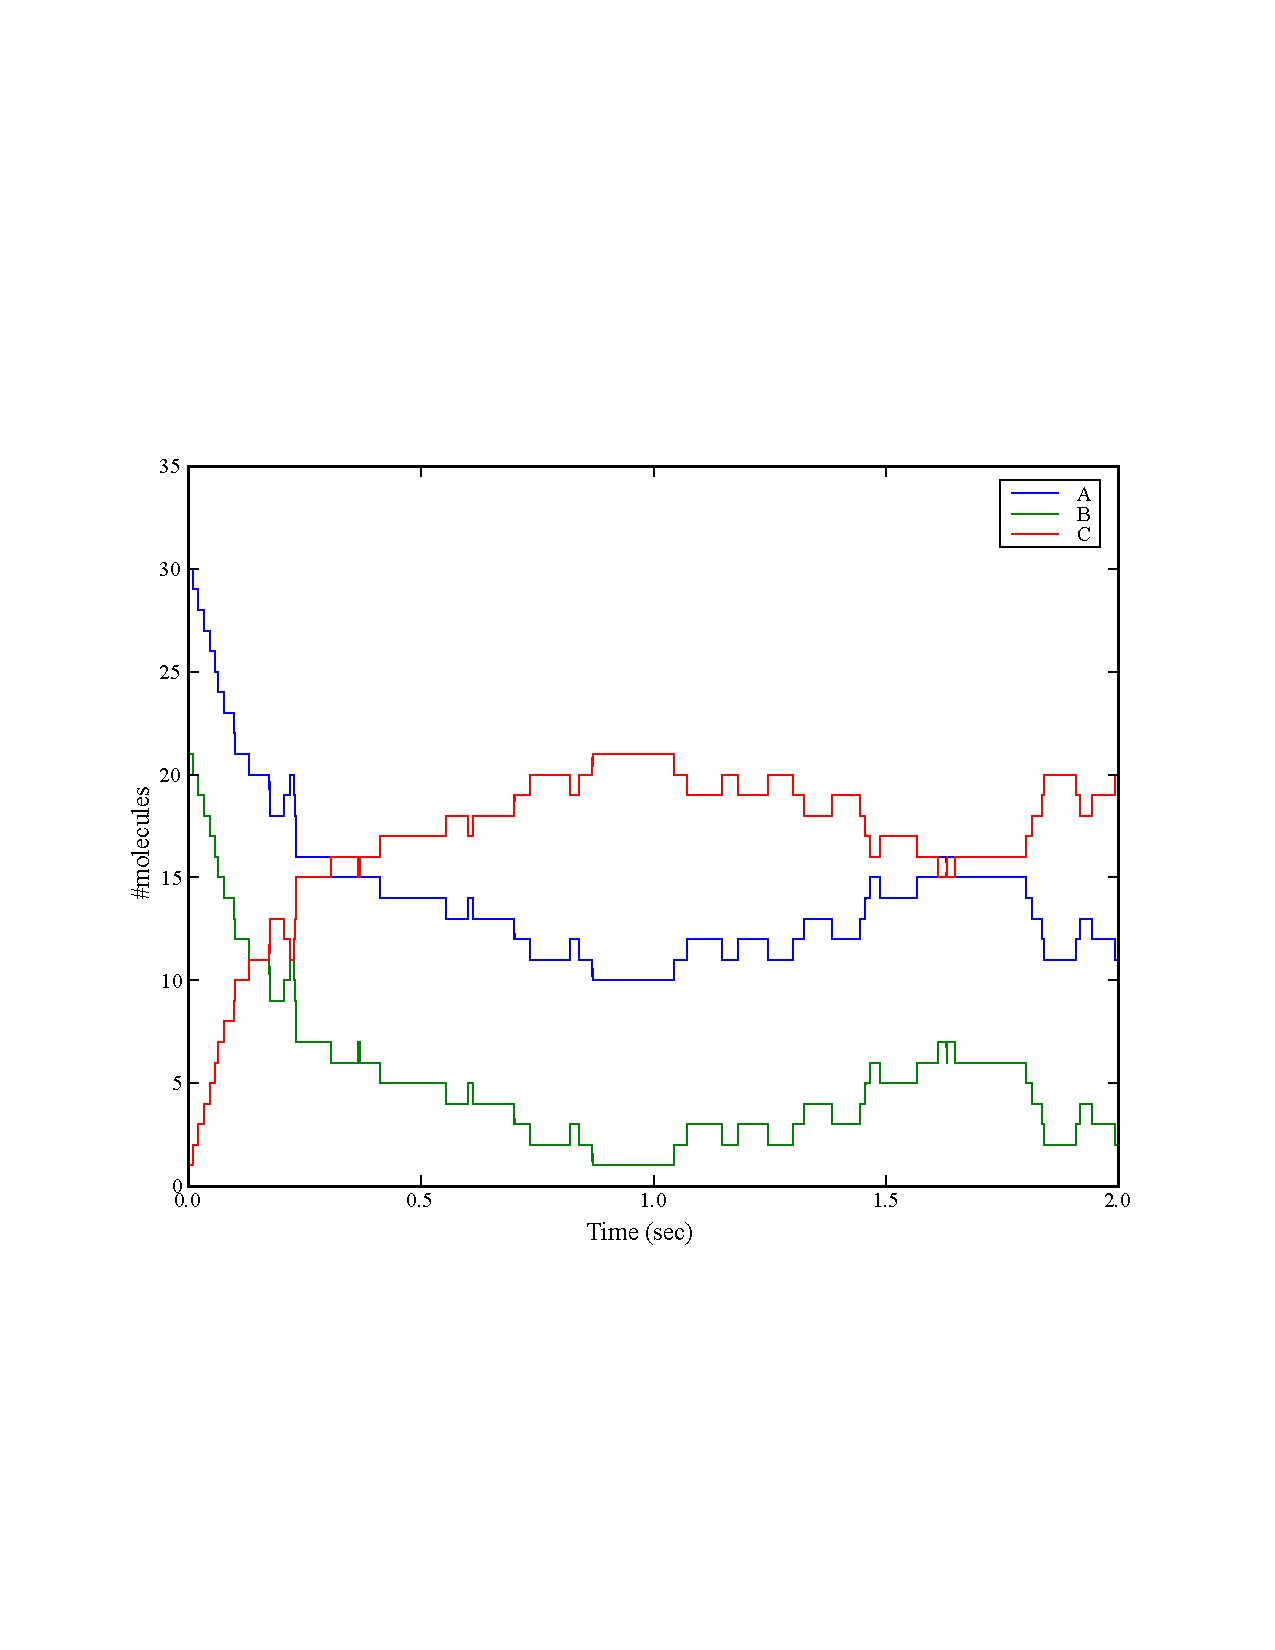
\includegraphics[width=13cm]{chap02_secondorderreaction01.pdf}
\caption{Simulating a single iteration of the second order reaction given in equation~\ref{eqn:secondorderreaction} with solver \texttt{wmdirect}. Because of the low numbers of molecules, we can clearly see the reactions occuring as discrete events.}
\label{fig:chap02:secondorderreaction01}
\end{figure}

If we're using a stochastic simulation algorithm such as that implemented in solver \texttt{wmdirect}, we're usually interested in analysing the range of behaviours produced by different iterations. One way of doing that is by taking the mean over multiple iterations, as is done in the following simulation code (result shown in figure~\ref{fig:chap02:secondorderreaction02}):

\begin{verbatim}
res = numpy.zeros([100,2001,3])
tpnt = numpy.arange(0.0, 2.001, 0.001)

for i in xrange(0,100):
    sim.reset()
    sim.setCompConc('comp', 'molA', 31.4e-6)
    sim.setCompConc('comp', 'molB', 22.3e-6)
    
    for t in xrange(0,2001):
        sim.run(tpnt[t])
        res[i,t,0] = sim.getCompCount('comp', 'molA')
        res[i,t,1] = sim.getCompCount('comp', 'molB')
        res[i,t,2] = sim.getCompCount('comp', 'molC')

res2 = numpy.mean(res, 0)

plot(tpnt, res2[:,0])
plot(tpnt, res2[:,1])
plot(tpnt, res2[:,2])
xlabel('Time (sec)')
ylabel('#molecules')
legend(('A','B','C'))
show()
\end{verbatim}

\begin{figure}
\centering
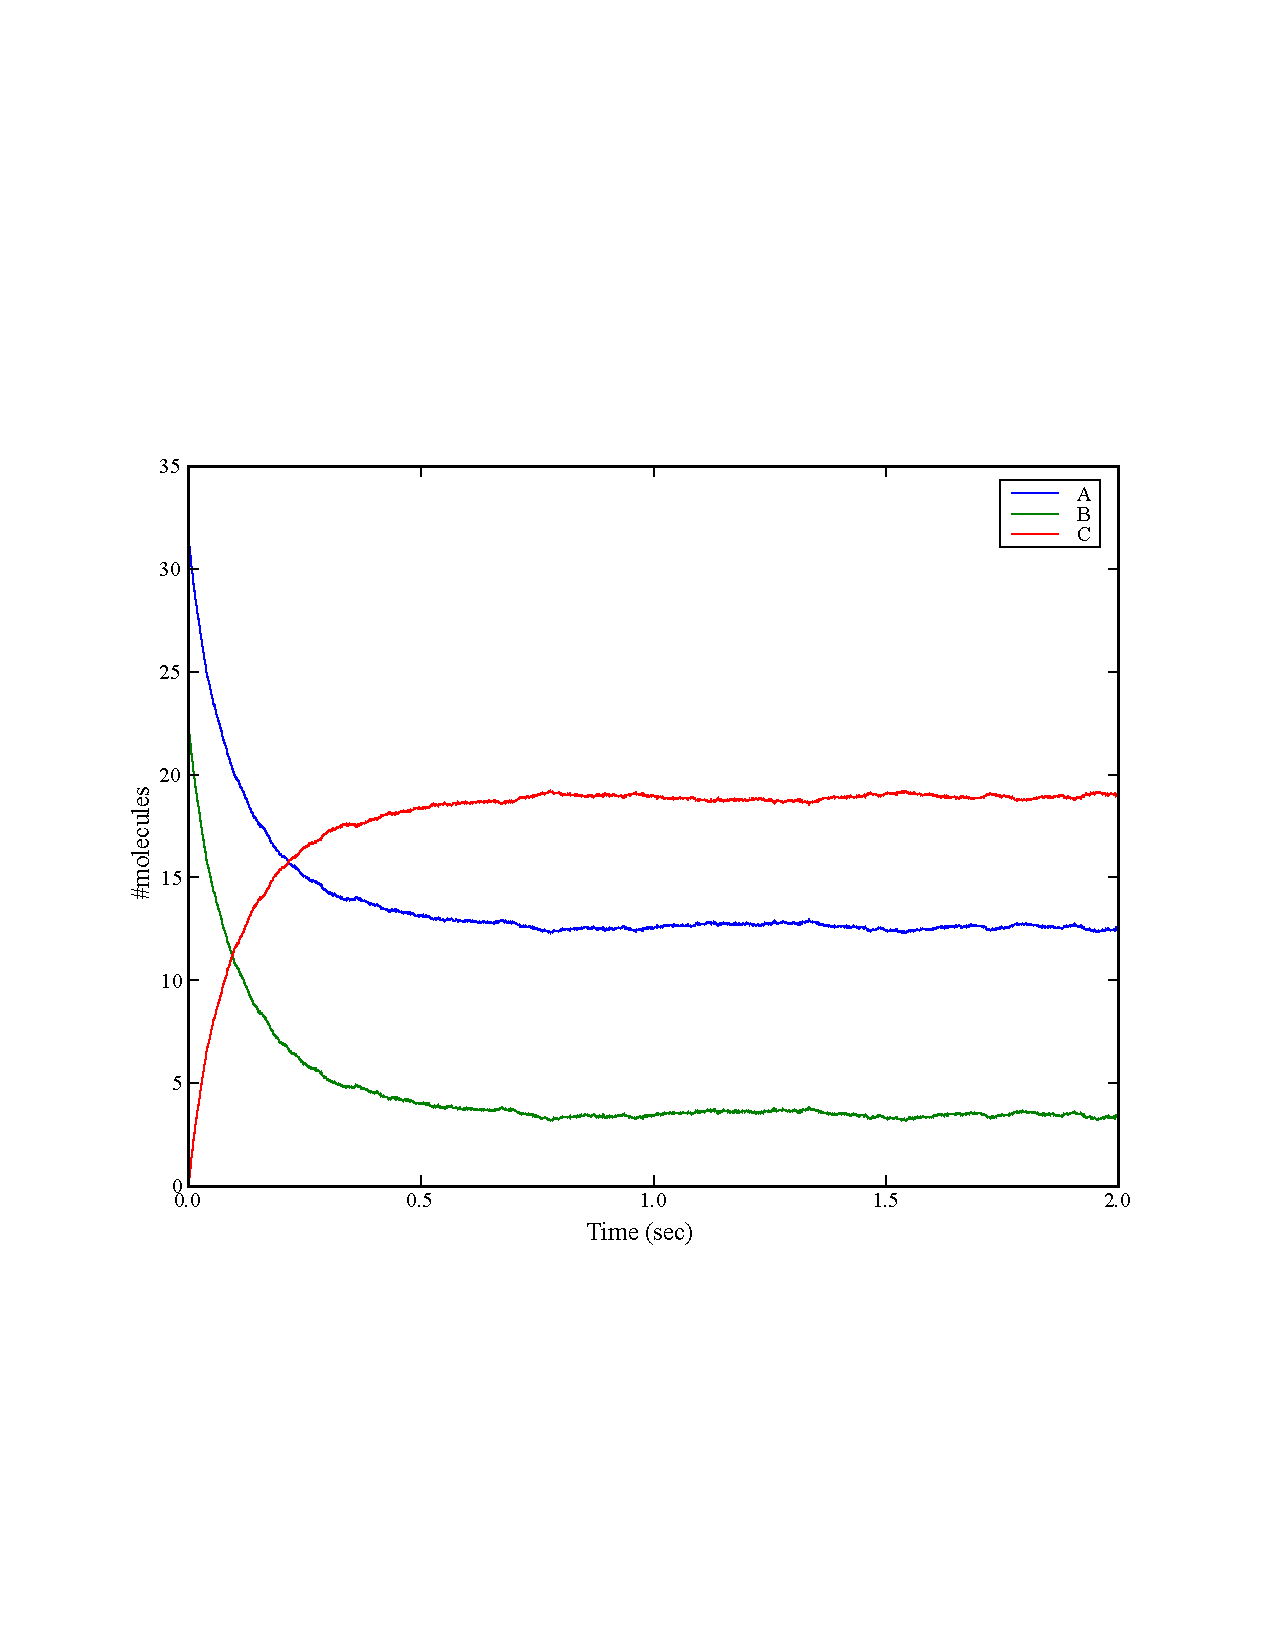
\includegraphics[width=13cm]{chap02_secondorderreaction02.pdf}
\caption{Average of multiple ($n=100$) iterations of the second order reaction given in equation~\ref{eqn:secondorderreaction}.}
\label{fig:chap02:secondorderreaction02}
\end{figure}

As you can see, the array that will be used to store the simulation results (array \texttt{res}) is now a three dimensional array, with the first dimension set to record 100 iterations. The loop that runs over all time points is now embedded in a loop that runs over the iterations. The \texttt{reset} function and the initial conditions are called at the beginning of each iteration. Since we don't need any detailed control over which iteration starts with which RNG seed value, we initialize the RNG just once, prior to anything else. Once the 100 iterations are done, we call NumPy's \texttt{mean} function to compute the mean over the first dimension, and then plot these mean values. 

\subsection{Controlling the simulation}

In the previous section, we stopped the simulation at regular time intervals to only record the concentrations of various molecules. The only time we actively \emph{changed} the simulation state was at $t=0$, to set the initial conditions. However, the function calls we used to set initial conditions can be called at any time during the simulation. 

As an example, let's interrupt our simulation at $t=1$ sec to add 10 molecules of species $A$. A single iteration of this simulation can be seen in figure~\ref{fig:chap02:secondorderreaction03}; the mean behaviour in figure~\ref{fig:chap02:secondorderreaction04}. 

\begin{verbatim}
for t in xrange(0,1001):
    sim.run(tpnt[t])
    res[i,t,0] = sim.getCompCount('comp', 'molA')
    res[i,t,1] = sim.getCompCount('comp', 'molB')
    res[i,t,2] = sim.getCompCount('comp', 'molC')
    
# Add 10 molecules of species A
sim.setCompCount('comp', 'molA', sim.getCompCount('comp', 'molA') + 10)

for t in xrange(1001,2001):
    sim.run(tpnt[t])
    res[i,t,0] = sim.getCompCount('comp', 'molA')
    res[i,t,1] = sim.getCompCount('comp', 'molB')
    res[i,t,2] = sim.getCompCount('comp', 'molC')
\end{verbatim}

\begin{figure}
\centering
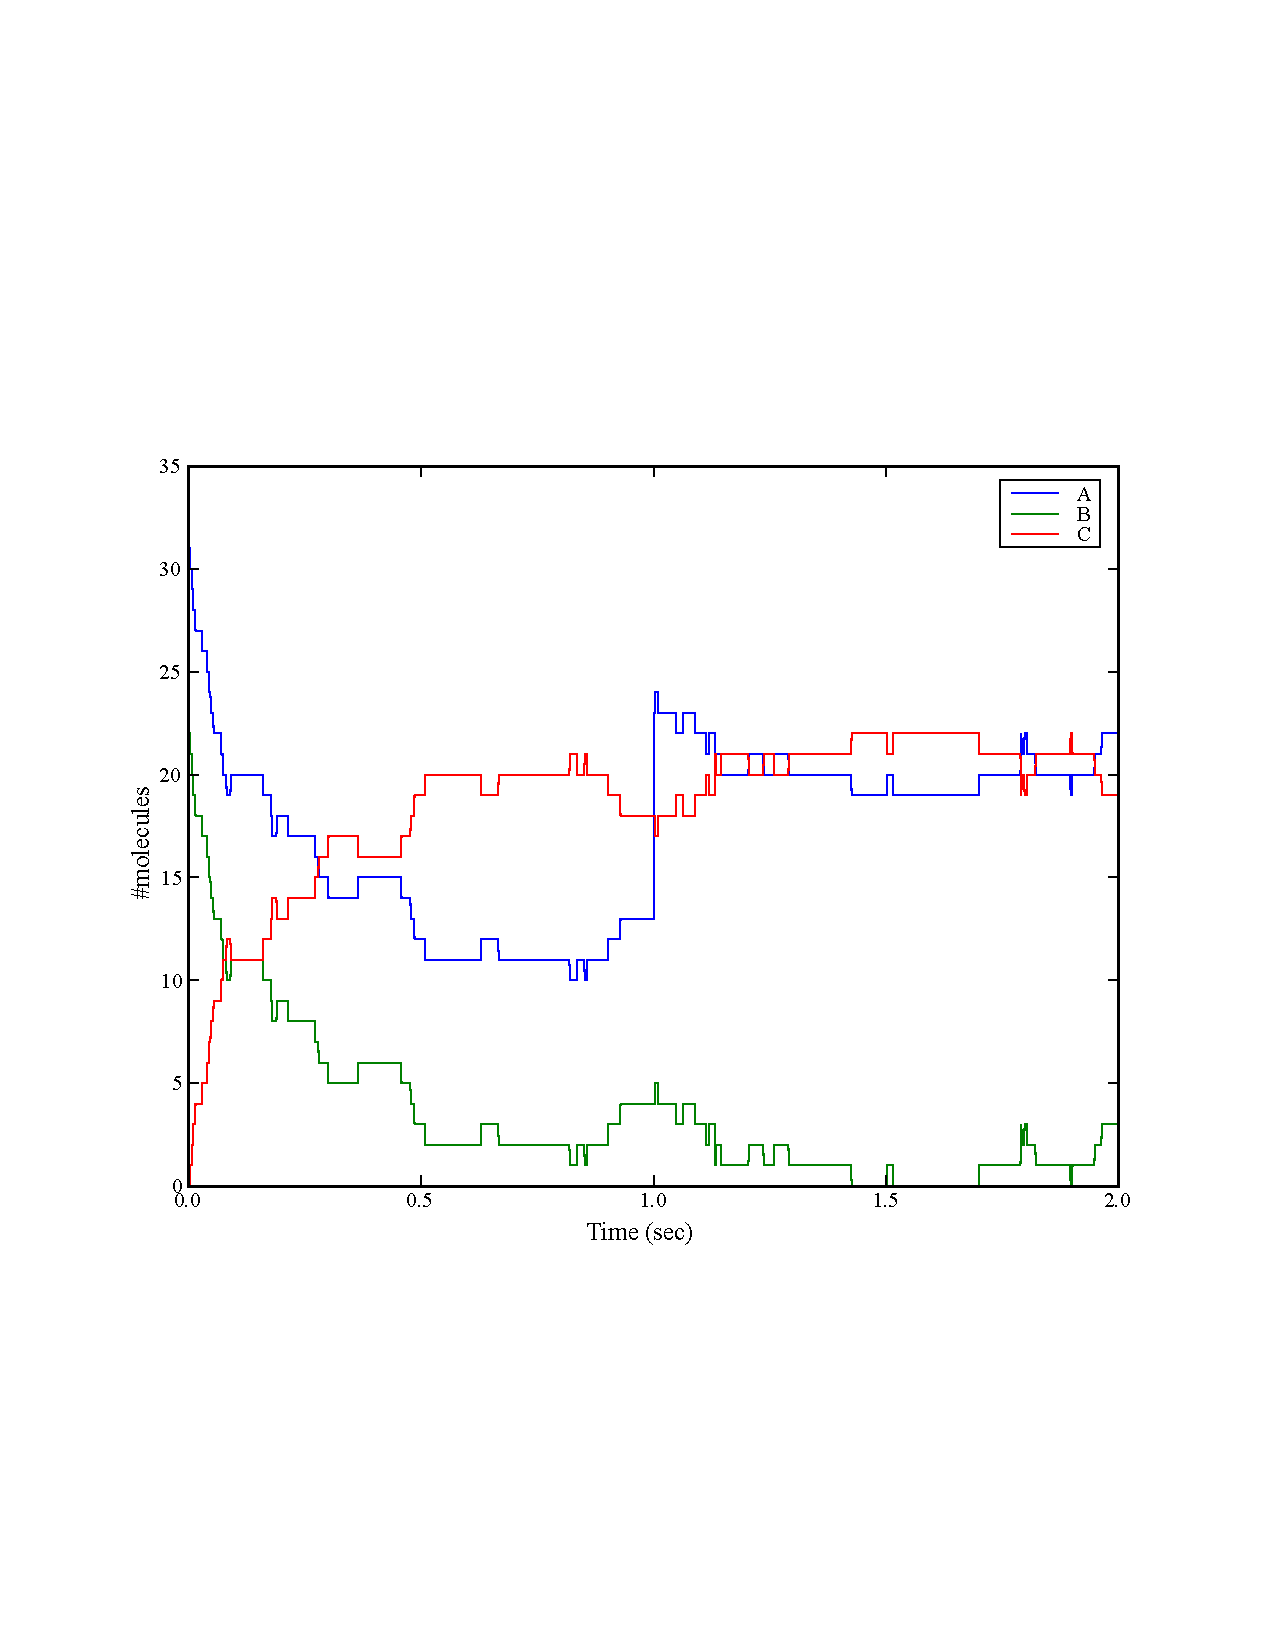
\includegraphics[width=13cm]{chap02_secondorderreaction03.pdf}
\caption{A single iteration of the second order reaction, with an injection of 10 molecules of species $A$ at $t=1.0$.}
\label{fig:chap02:secondorderreaction03}
\end{figure}

\begin{figure}
\centering
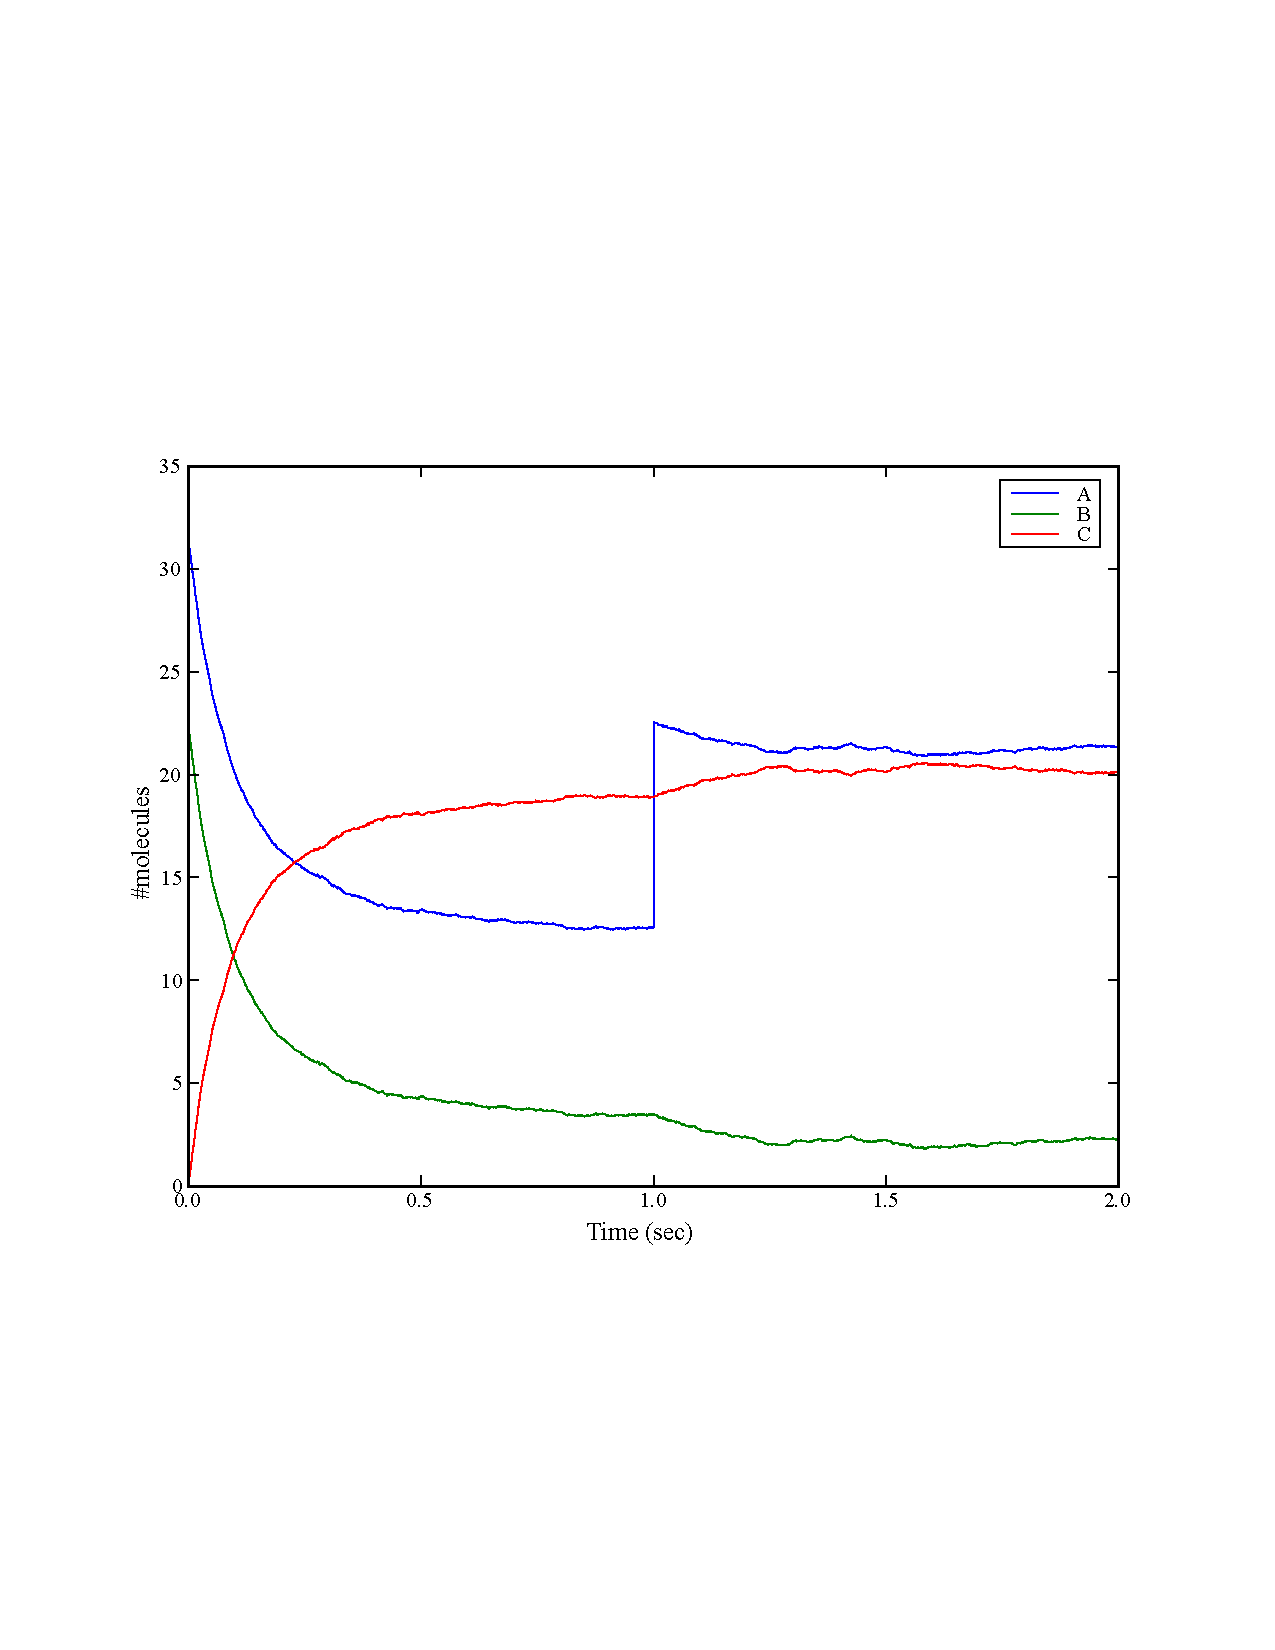
\includegraphics[width=13cm]{chap02_secondorderreaction04.pdf}
\caption{The mean of multiple ($N=100$) iterations of the second order reaction, with an injection of 10 molecules of species $A$ at $t=1.0$.}
\label{fig:chap02:secondorderreaction04}
\end{figure}

When you have to do these things regularly, you might want to encapsulate various parts of this code in separate functions to save yourself some coding time. 

Quite often, one does not want to simulate the sudden injection of molecules, but rather keep the concentration of some species constant at a controlled value. This means that any reaction involving the buffered molecule will still occur if the reactants are present in sufficiently large numbers, but the occurrence of this reaction will not actually change the amount of the buffered species that is present. The following code snippet shows how, during the time interval $0.1 \leq t < 0.6$, the concentration of species $A$ is clamped to whatever its value was at $t = 0.5$.\footnote{This way of using the compartmental buffering mechanism will not often be used in a real simulation; more often clamping will be combined with a call to \texttt{setCompCount} or one of its variants.} Results can be seen in figure~\ref{fig:chap02:secondorderreaction05} for a single iteration and \ref{fig:chap02:secondorderreaction06} for the mean of multiple iterations.

\begin{verbatim}
for t in xrange(0,101):
    sim.run(tpnt[t])
    res[i,t,0] = sim.getCompCount('comp', 'molA')
    res[i,t,1] = sim.getCompCount('comp', 'molB')
    res[i,t,2] = sim.getCompCount('comp', 'molC')
    
sim.setCompClamped('comp', 'molA', True)

for t in xrange(101,601):
    sim.run(tpnt[t])
    res[i,t,0] = sim.getCompCount('comp', 'molA')
    res[i,t,1] = sim.getCompCount('comp', 'molB')
    res[i,t,2] = sim.getCompCount('comp', 'molC')
    
sim.setCompClamped('comp', 'molA', False)

for t in xrange(601,2001):
    sim.run(tpnt[t])
    res[i,t,0] = sim.getCompCount('comp', 'molA')
    res[i,t,1] = sim.getCompCount('comp', 'molB')
    res[i,t,2] = sim.getCompCount('comp', 'molC')
\end{verbatim}

\begin{figure}
\centering
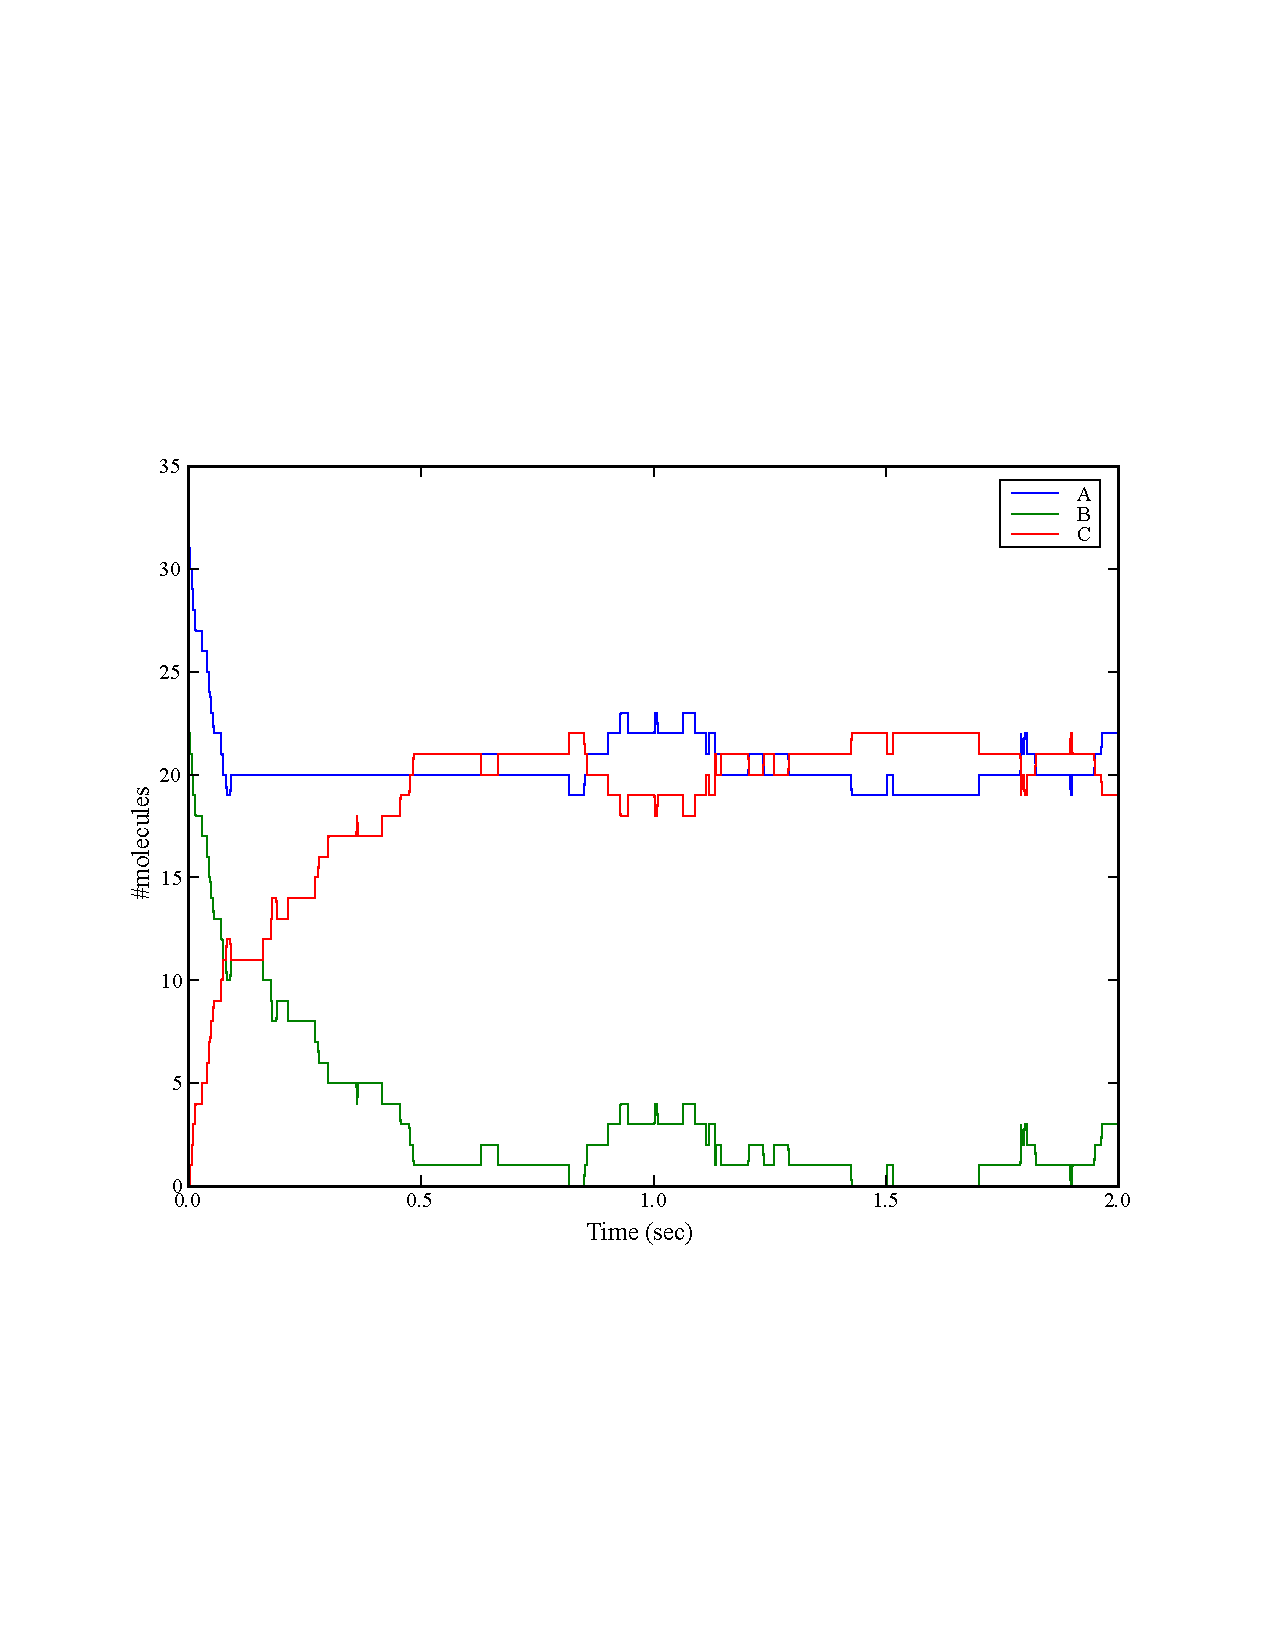
\includegraphics[width=13cm]{chap02_secondorderreaction05.pdf}
\caption{A single iteration of the second order reaction, where the concentration of $A$ is clamped during the interval $0.1 \leq t < 0.6$.}
\label{fig:chap02:secondorderreaction05}
\end{figure}

\begin{figure}
\centering
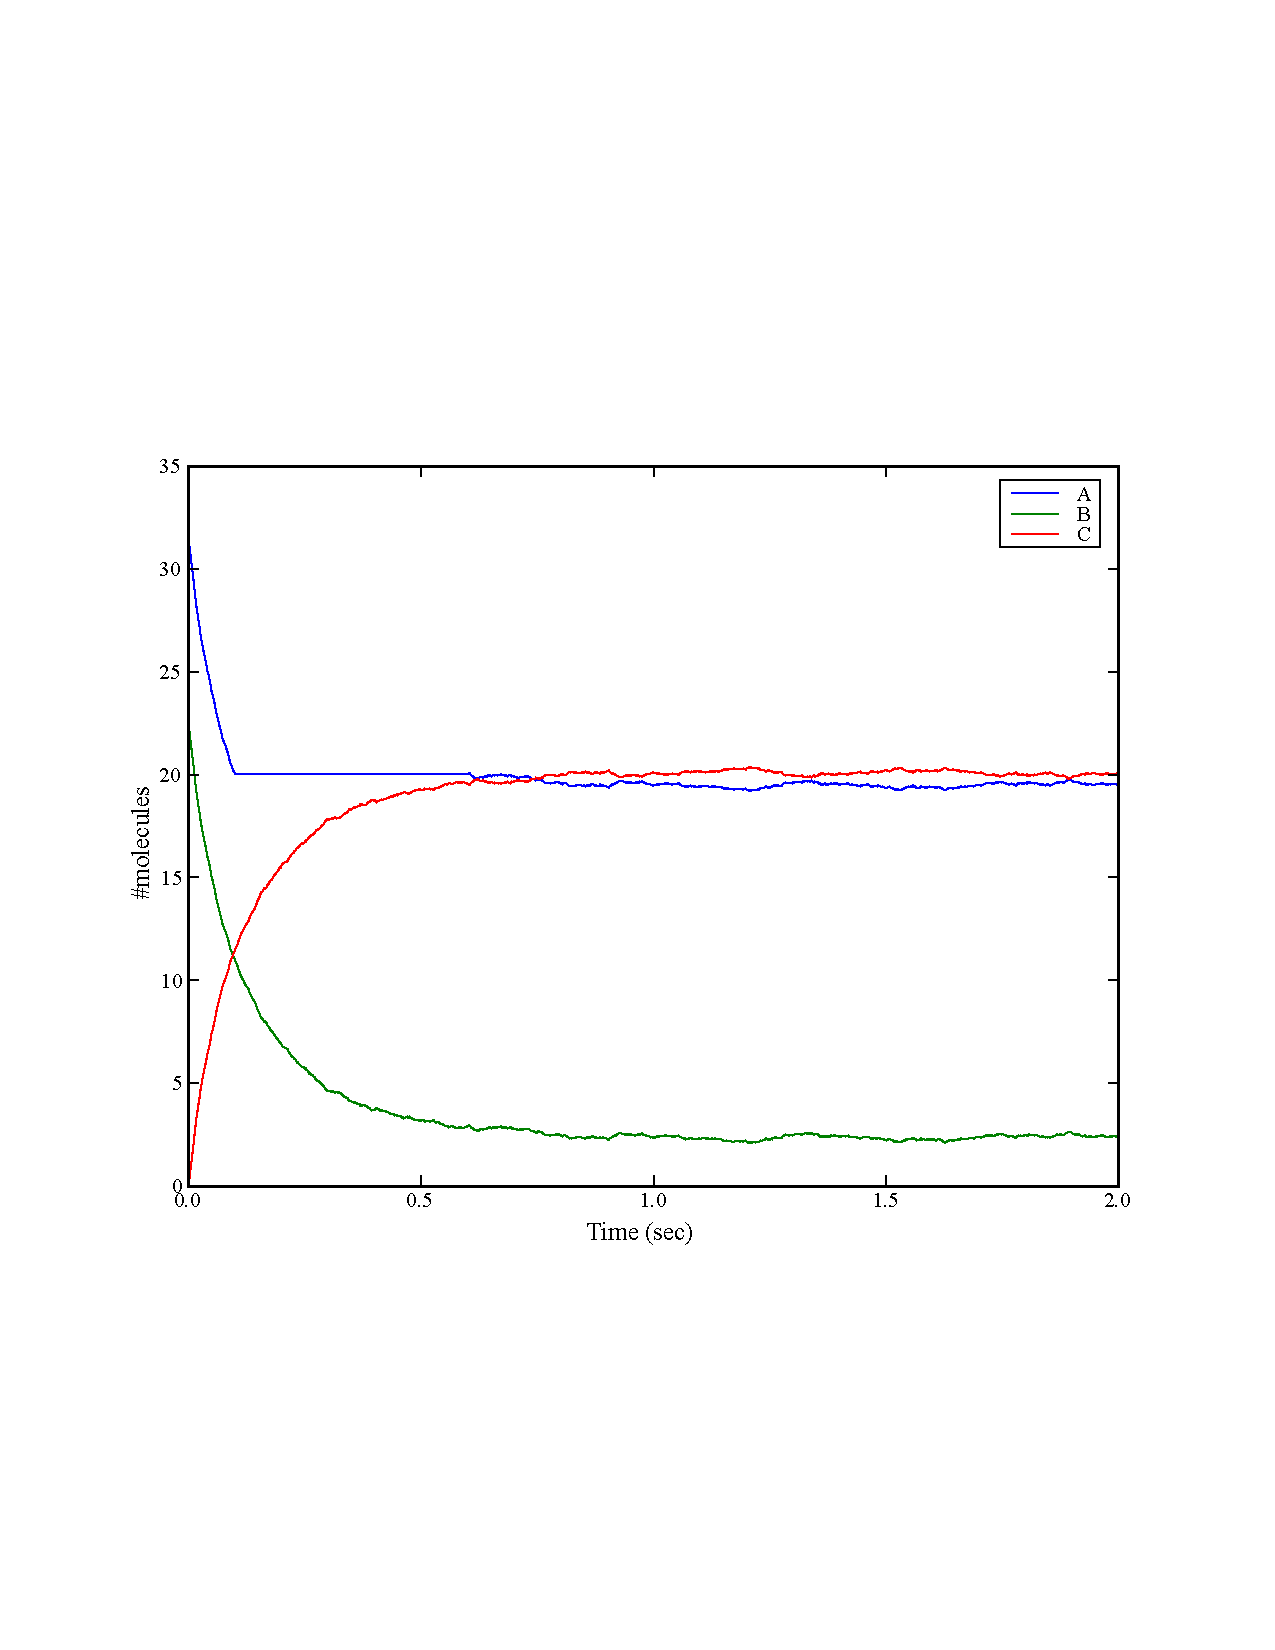
\includegraphics[width=13cm]{chap02_secondorderreaction06.pdf}
\caption{The mean of multiple ($N=100$) iterations of the second order reaction, where the concentration of $A$ is clamped during the interval $0.1 \leq t < 0.6$.}
\label{fig:chap02:secondorderreaction06}
\end{figure}

The function \texttt{setCompClamped} takes a boolean which is used to turn on or off the clamping of the species in the specified compartment. 

A final way in which we will control our simulation in this chapter is by activating/inactivating a reaction channel. Inactivating a reaction channel means that it will never occur, regardless of whether the required reactants are present in sufficient numbers. In the following simulation: 
\begin{itemize}
\item we will turn off the forward reaction of equation~\ref{eqn:secondorderreaction} during interval $2.0 \leq t < 4.0$;
\item turn it back on and let everything recover during $4.0 \leq t < 6.0$;
\item turn off the backward reaction during $6.0 \leq t < 8.0$; 
\item turn it back on and let everything recover again during $8.0 \leq t < 10.0$;
\item and finally turn off both the forward and backward channel during a final interval $10.0 \leq t < 12.0$.
\end{itemize}
This time, we'll wrap the run-until-time-$t$ part of the code in a separate function to save ourselves some writing:
\begin{verbatim}
def run(i, tp1, tp2):
    for t in xrange(tp1,tp2):
        sim.run(tpnt[t])
        res[i,t,0] = sim.getCompCount('comp', 'molA')
        res[i,t,1] = sim.getCompCount('comp', 'molB')
        res[i,t,2] = sim.getCompCount('comp', 'molC')
\end{verbatim} 

The actual simulation code now becomes:
\begin{verbatim}
run(i,0,2001)
sim.setCompReacActive('comp', 'kreac_f', False)
run(i,2001,4001)
sim.setCompReacActive('comp', 'kreac_f', True)
run(i,4001,6001)
sim.setCompReacActive('comp', 'kreac_b', False)
run(i,6001,8001)
sim.setCompReacActive('comp', 'kreac_b', True)
run(i,8001,10001)
sim.setCompReacActive('comp', 'kreac_f', False)
sim.setCompReacActive('comp', 'kreac_b', False)
run(i,10001,12001)
\end{verbatim}
The results of this code can be seen in figures~\ref{fig:chap02:secondorderreaction07} and~\ref{fig:chap02:secondorderreaction08}.

\begin{figure}
\centering
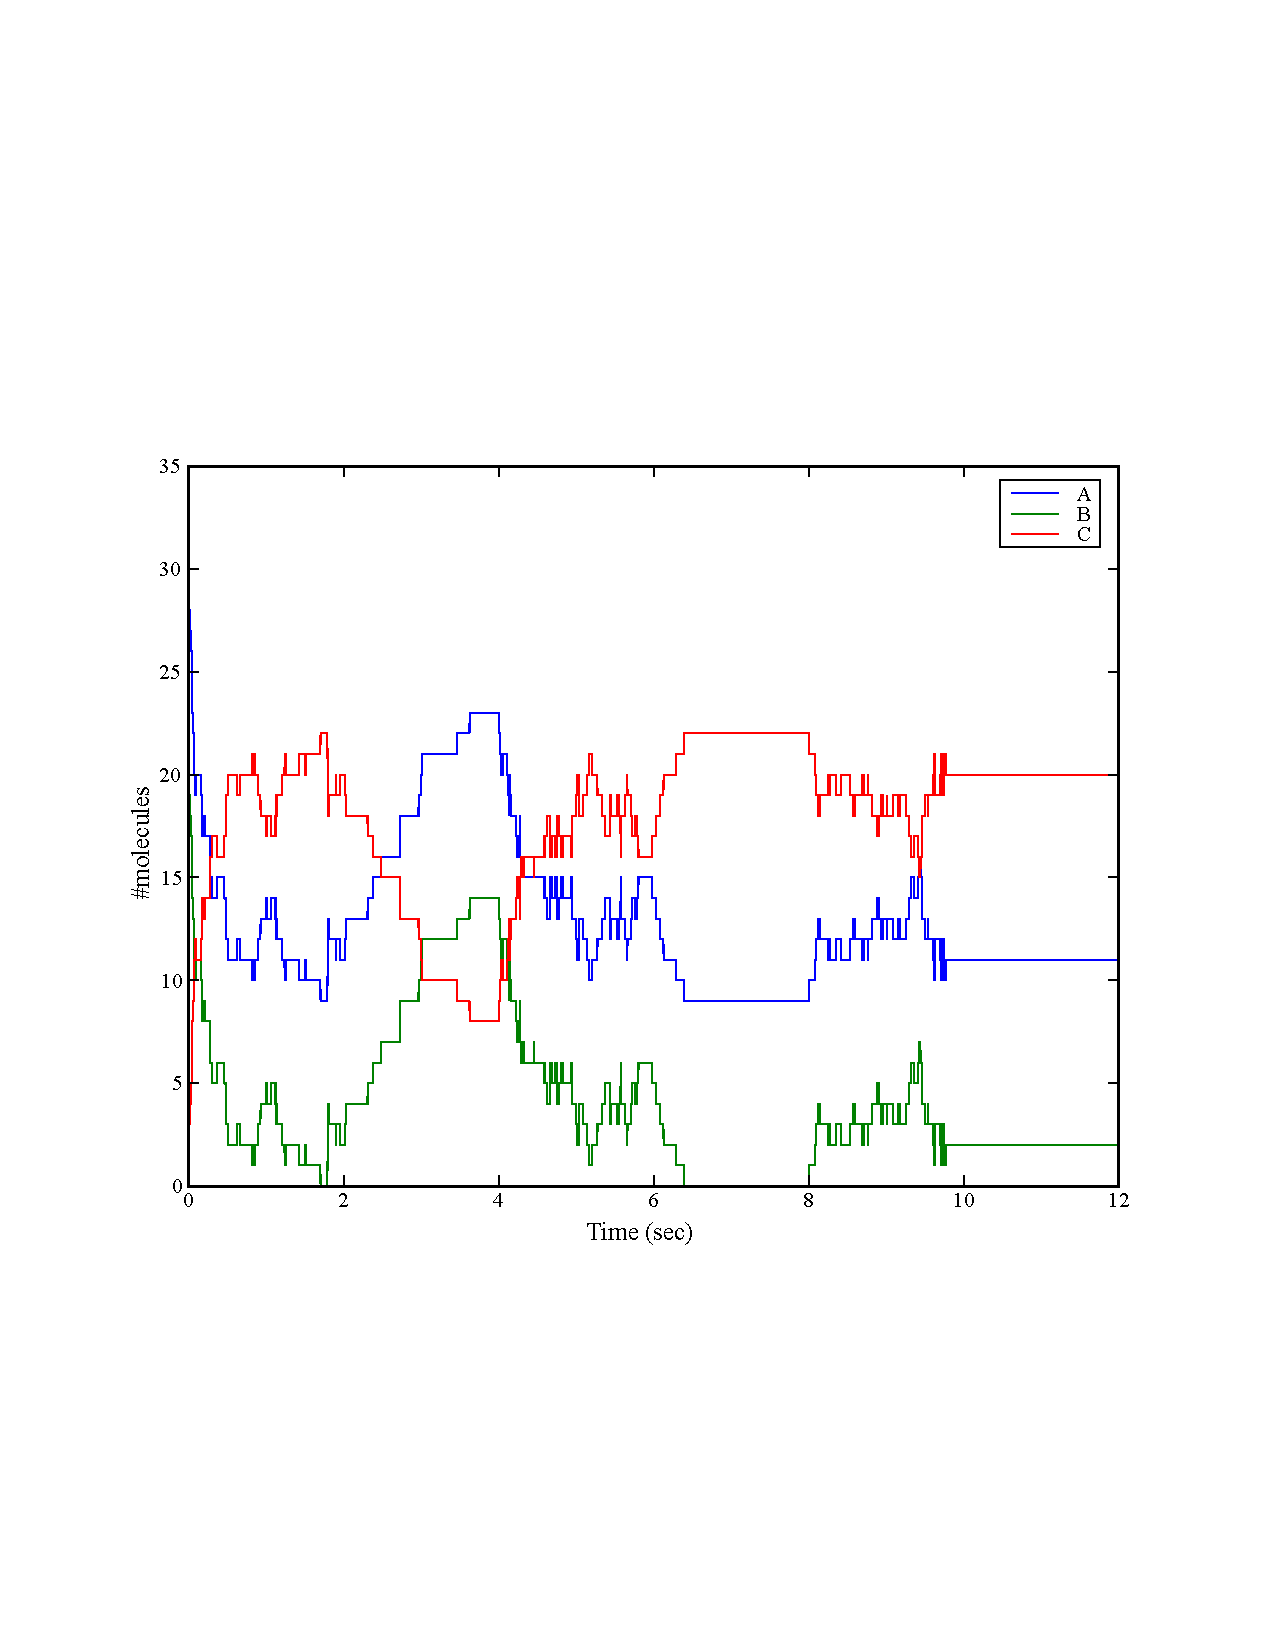
\includegraphics[width=13cm]{chap02_secondorderreaction07.pdf}
\caption{A single iteration of the second order reaction, with the forward and backward reaction turned on and off.}
\label{fig:chap02:secondorderreaction07}
\end{figure}

\begin{figure}
\centering
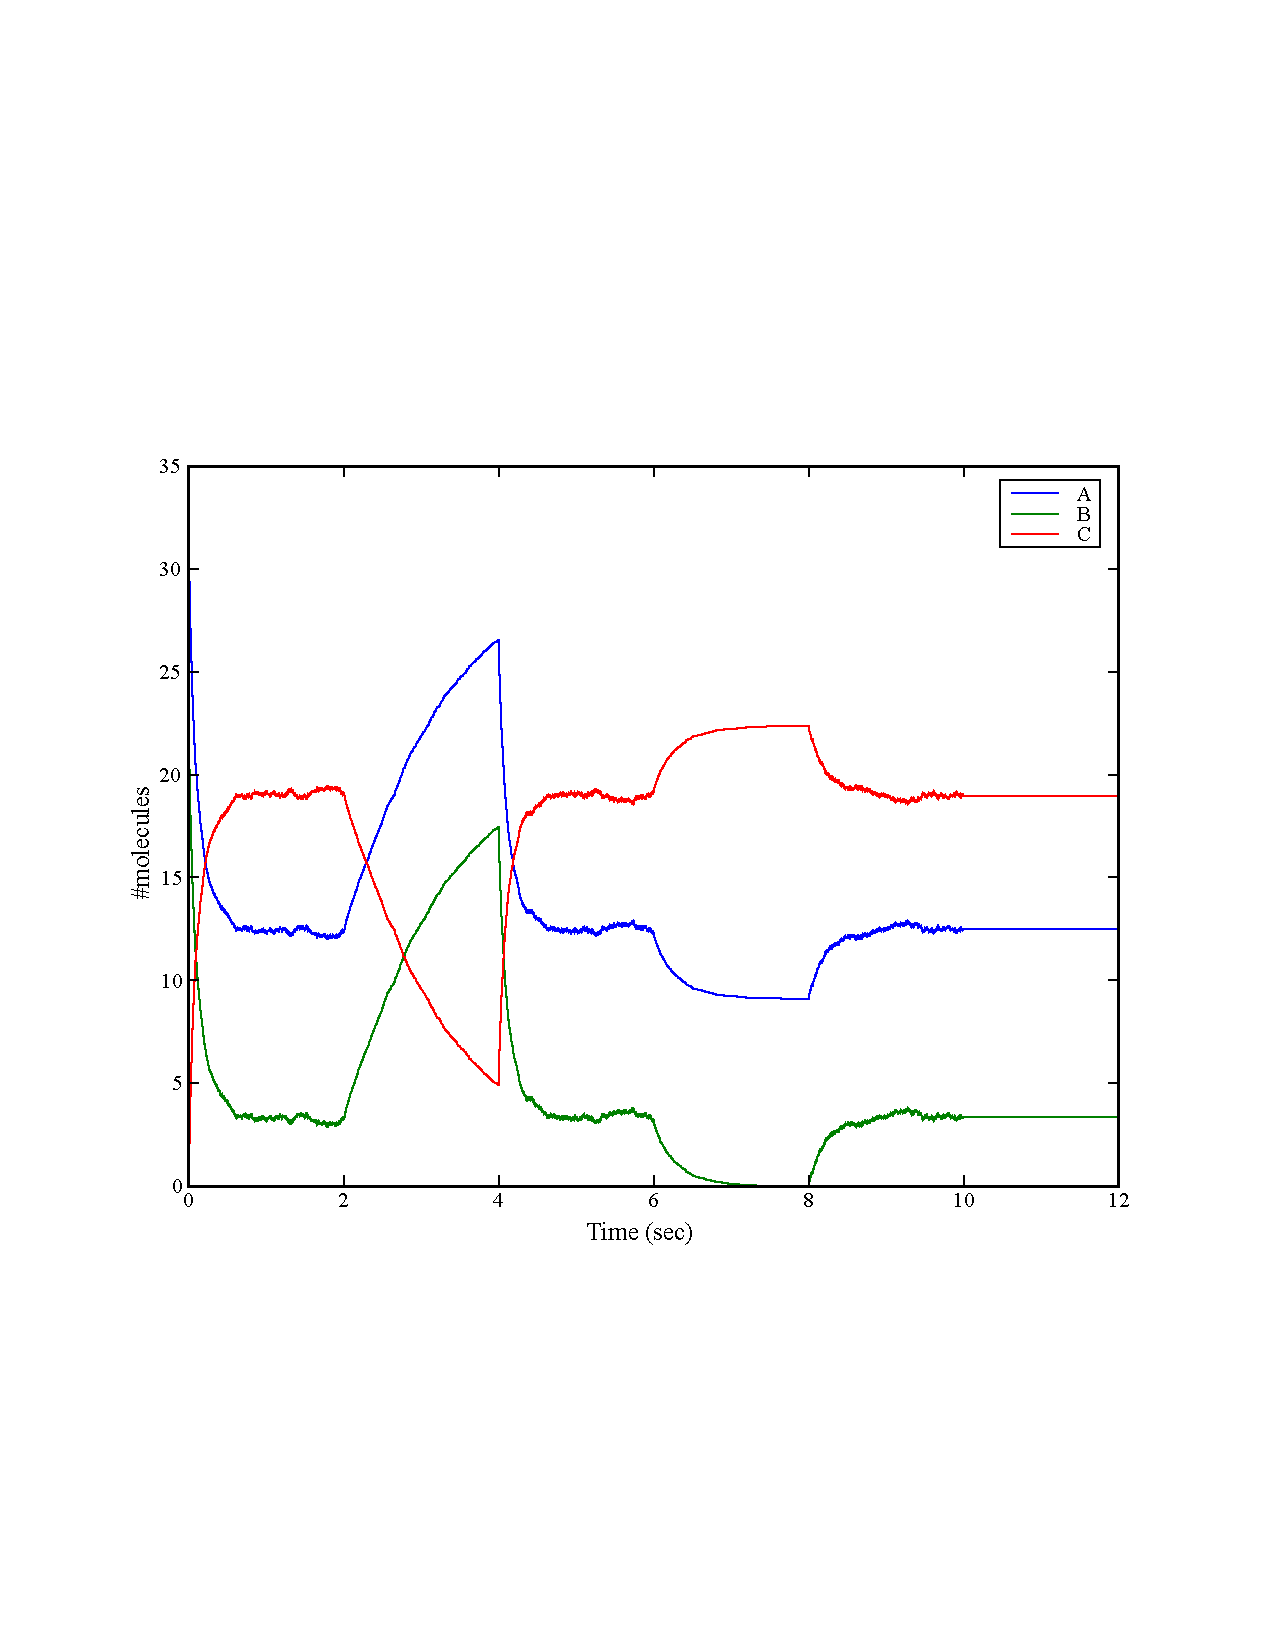
\includegraphics[width=13cm]{chap02_secondorderreaction08.pdf}
\caption{The mean of multiple ($N=100$) iterations of the second order reaction, with the forward and backward reaction turned on and off.}
\label{fig:chap02:secondorderreaction08}
\end{figure}

\section{The Lotka-Volterra system}

This section will cover much of the same material from the previous one, but applied to a slightly larger reaction system: the Lotka-Volterra system. Will show how to enforce non-standard reaction constants.

To be added.

% % % % % % % % % % % % % % % % % % % % % % % % % % % % % % % % % % % % % % % % 
\chapter{Surface-volume reactions}

% % % % % % % % % % % % % % % % % % % % % % % % % % % % % % % % % % % % % % % % 
\chapter{An \inspt\ receptor model}

% % % % % % % % % % % % % % % % % % % % % % % % % % % % % % % % % % % % % % % % 
\chapter{Simulating diffusion}\label{chap:simulatingdiffusion}

This chapter introduces modeling and simulation of diffusion systems. We start by explaining how the diffusive motion of one or more molecules can be described in \texttt{steps.model} models. Next, we describe a few examples of simulating diffusion and reaction-diffusion systems using solver \texttt{tetexact}, which is an extension of solver \texttt{wmdirect} which was introduced in Chapter~\ref{chap:wmkinetics}. Since \texttt{tetexact} requires a tetrahedral mesh, this chapter also briefly introduces working with these objects. A more detailed explanation on the use and, more importantly, the construction of such meshes is explained in another chapter.

\section{A simple diffusion system}

As usual, we begin with a simple problem. In this case, we will simulate the diffusion of molecules of a single species, called $A$, in a simple stretched-out bar of length 20~$\mu m$. At $t=0$, we inject the molecules in the middle of the bar and let them diffuse towards equilibrium. Let's assume that the diffusion constant of $A$, $D_{A}$, is 0.08~$\mu m^{2}ms^{-1}$, for no particular reason.\footnote{0.08~$\mu m^{2}ms^{-1}$ is actually the diffusion constant of dextran in the cytosol.}

\subsection{PDE solution}

Before we perform this simulation with STEPS, let's have quick peak at the results that we will expect STEPS to produce, by integrating the diffusion equation numerically. For simplicity, we will solve the PDE for only 1 spatial dimension, even though the actual STEPS simulation will work in 3 dimensions. The PDE is of course given by the diffusion equation:

\begin{equation}\label{eqn:simplediffusion01}
\frac{\partial A(x,t)}{\partial t} = D_A \cdot \frac{\partial^2 A(x,t)}{\partial x^2}
\end{equation}

$A(x,t)$ refers to the concentration of $A$ at position $x$ and time $t$. Since we will simulate diffusion in a bar of limited length, we need to make sure that we have reflective boundary conditions at the end points of the bar. This is expressed with the following Neumann boundary conditions:

\begin{equation}\label{eqn:simplediffusion02}
\left.\frac{\partial A(x,t)}{\partial x} = 0\ \right|_{x=-10,+10\ \mu m}
\end{equation}

Our initial condition consists of the following: 

\begin{equation}\label{eqn:simplediffusion03}
A(x,0) =
\left\{
\begin{aligned}
A_0 \quad & x \in [-0.1\ \mu m,\ +0.1\ \mu m]\\
0 \quad & \text{otherwise}
\end{aligned}
\right.
\end{equation}

In Figure~\ref{fig:simplediffusion01}, we can see the solution of this problem for different times, for $t$ going up to 640 $ms$, at which point it has almost reached equilibrium. We can also measure the apparent diffusion constant $D_\text{app}$ by computing the change in $\left< x^2 \right> / 2 t$ over time. This is plotted in Figure~\ref{fig:simplediffusion02}. For diffusion in an infinite space, $D_\text{app}$ would be equal to 0.08~$\mu m^{2}ms^{-1}$ for every time. In Figure~\ref{fig:simplediffusion02}, however, we see that $D_\text{app}$ starts to fall sharply somewhere around $t = 100\ ms$. This is of course caused by our reflective boundary conditions, which start to exert a increasingly large influence on the diffusion process around that point in time.\footnote{Furthermore, $D_\text{app}$ is slightly larger than 0.08~$\mu m^{2}ms^{-1}$ in the first few milliseconds, because our initial condition was not a Dirac delta function but a square pulse.}

\begin{figure}
\centering
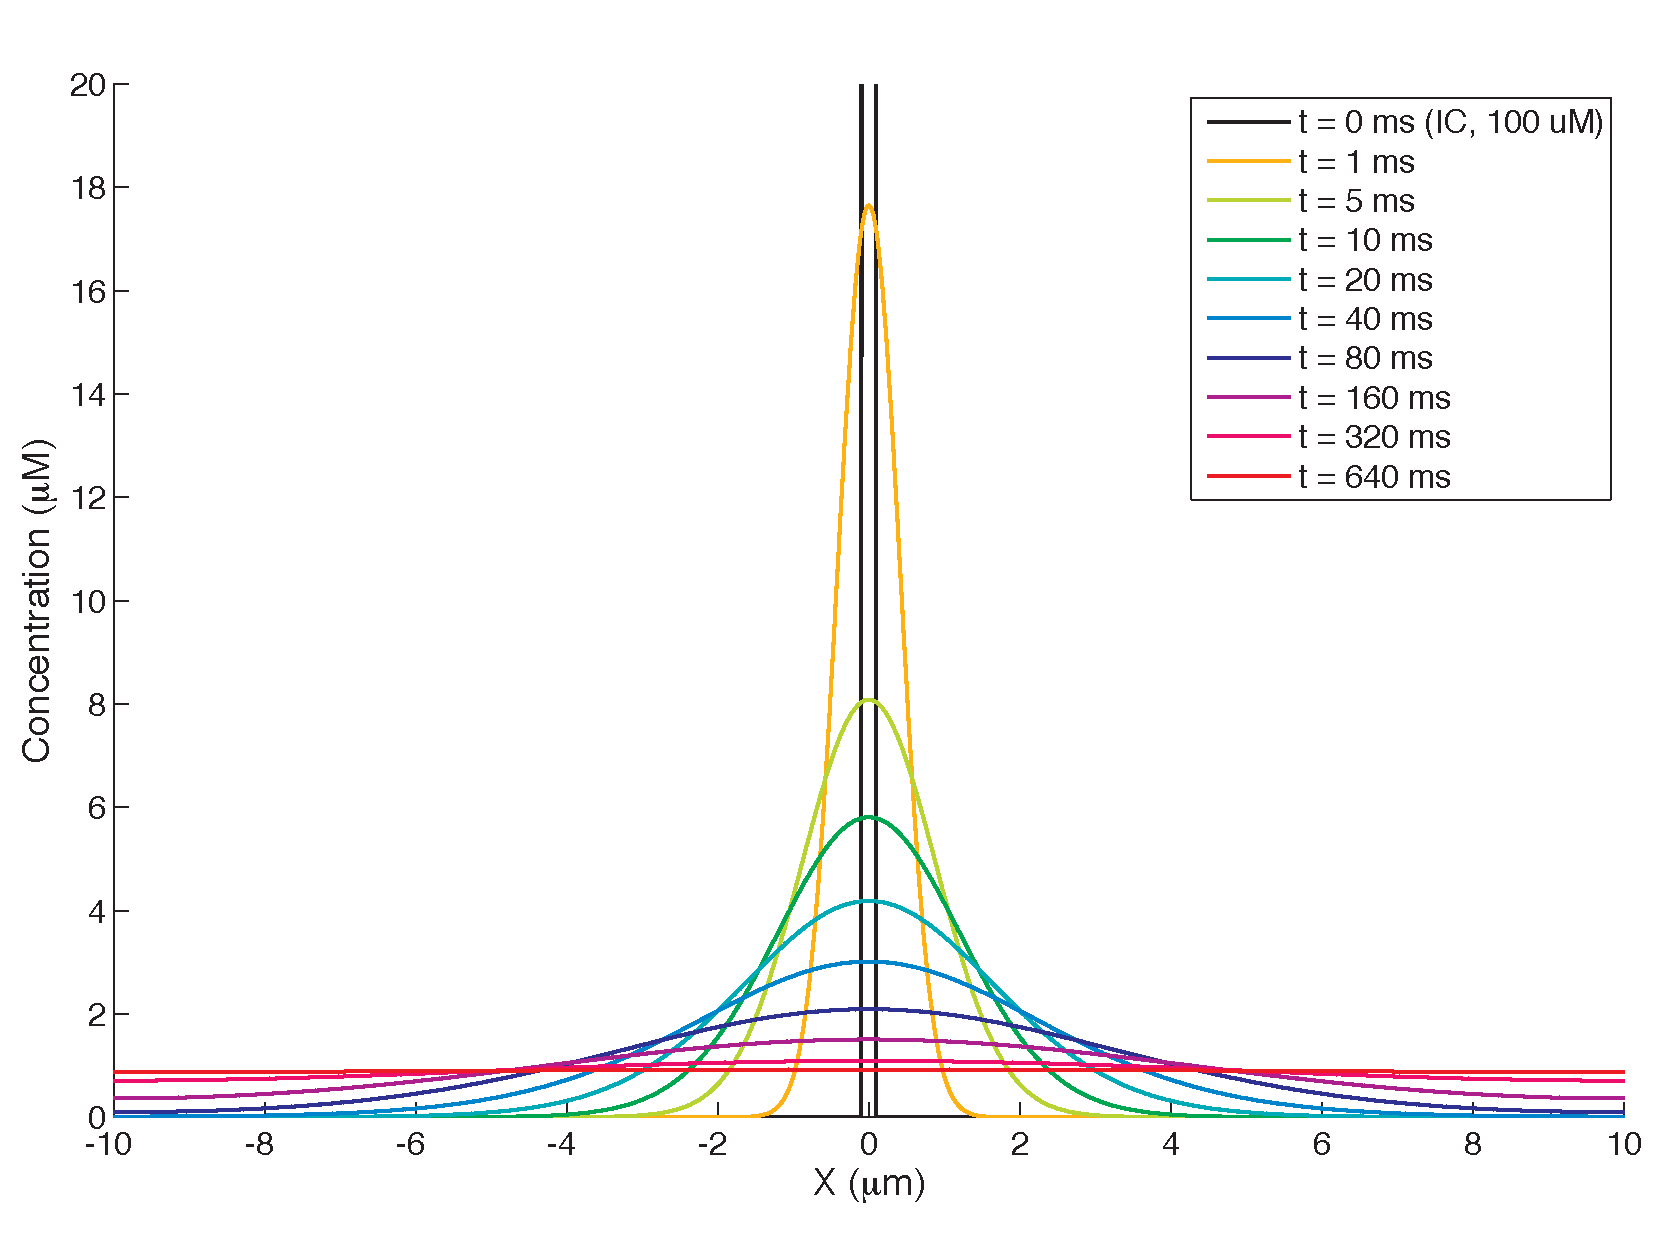
\includegraphics[width=13cm]{simplediffusion01.pdf}
\caption{Solution for Equation~\ref{eqn:simplediffusion01} with the boundary conditions specified in Equation~\ref{eqn:simplediffusion02} and the initial condition of Equation~\ref{eqn:simplediffusion03}.}
\label{fig:simplediffusion01}
\end{figure}

\begin{figure}
\centering
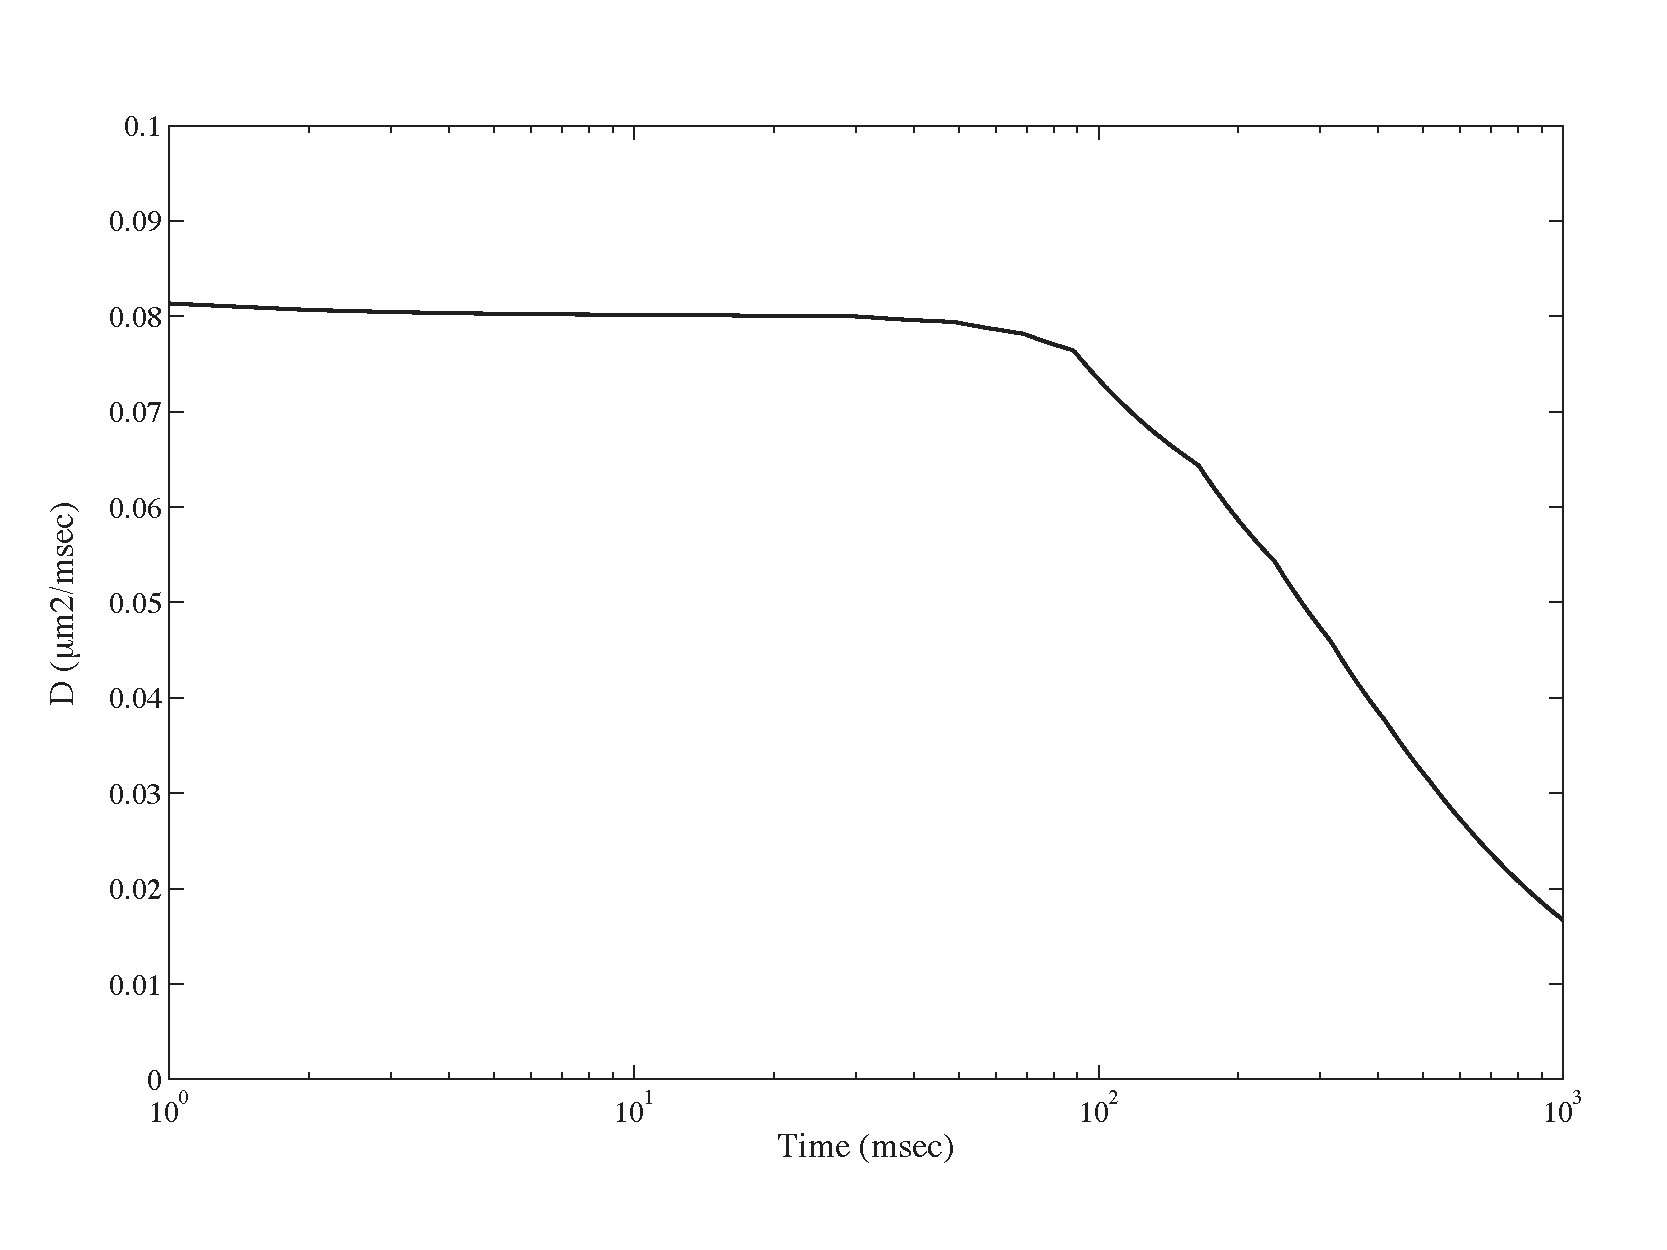
\includegraphics[width=13cm]{simplediffusion02.pdf}
\caption{Apparent diffusion constant, $D_\text{app}$, measured over time for the simulation in Figure~\ref{fig:simplediffusion01}.}
\label{fig:simplediffusion02}
\end{figure}

\subsection{Modeling diffusion}
When specifying your model in STEPS, adding diffusion rules for various  is very simple. It basically consists of nothing more 

% % % % % % % % % % % % % % % % % % % % % % % % % % % % % % % % % % % % % % % % 
\chapter{The \inspt\ receptor model in 3D}

% % % % % % % % % % % % % % % % % % % % % % % % % % % % % % % % % % % % % % % % 
\appendix

\chapter{Solver functions}\label{app:solverfunctions}

This appendix contains an overview of the function blocks that are implemented by the solvers implemented in STEPS.

\section{Function block: \texttt{core}}\label{app:solverfunctions:core}

\subsection{General functions}
{\setlength{\parskip}{12pt} \setlength{\parindent}{0pt}

\texttt{reset()}

Resets the simulation. The concentrations of all species in all simulation elements (whether tetrahedrons/triangles or whole compartments/patches) are set to zero. Reaction/diffusion constants are set to their model default values. The current time is reset to zero.

\texttt{run(endtime)}

Advance the simulation until time \texttt{endtime} is reached. Obviously, \texttt{endtime} must be larger or equal to the current time.

\texttt{getTime()}

Returns the current time of the simulation.
}

\subsection{Access to compartments}
{\setlength{\parskip}{12pt} \setlength{\parindent}{0pt}

\texttt{getCompVol(comp)}\\
\texttt{setCompVol(comp, vol)}

\texttt{getCompVol} returns the volume of the compartment with id \texttt{comp}. \texttt{setCompVol} sets the volume of the compartment with id \texttt{comp} to \texttt{vol}, expressed in SI units ($m^3$)\footnote{This would a cheap way of simulating structural changes to the reaction volume.}. Currently, \texttt{setCompVol} is not implemented in any solver.

\texttt{getCompCount(comp, spec)}\\
\texttt{setCompCount(comp, spec, n)}

\texttt{getCompCount} returns the amount of molecules (a positive integer) of a species with name \texttt{spec} in compartment \texttt{comp}.
\texttt{setCompCount} sets the amount of molecules of a species in a compartment to \texttt{n}, a positive integer argument. If the solver operates on a mesh, the molecules are uniformly distributed over the mesh elements that comprise the compartment.

\texttt{getCompAmount(comp, spec)}\\
\texttt{setCompAmount(comp, spec, a)}

\texttt{getCompAmount} returns the amount of molecules of a species with name \texttt{spec} in compartment \texttt{comp}. The value is returned in units of mol. \texttt{setCompAmount} sets the amount of molecules in a compartment, using the same unit (mol). When using a discrete solver, such as \texttt{wmdirect} or \texttt{tetexact}, this continuous value is converted internally into the number of molecules $N_{\mathrm{spec}}'$ by multiplication with Avogadro's number. To ``stochastically eliminate'' the fractional part, a uniform random number $u$ is generated in the range $[0,1)$ and $N_{\mathrm{spec}}'$ is rounded up or down as follows:
\begin{equation}
\label{eqn:stochfracrounding}
N_{\mathrm{spec}} = 
\begin{cases}
\lfloor N_{\mathrm{spec}}' \rfloor & \text{if } u \geq \text{frac}(N_{\mathrm{spec}}') \\
\lceil N_{\mathrm{spec}}' \rceil & \text{if } u < \text{frac}(N_{\mathrm{spec}}')
\end{cases}
\end{equation}
This means that the final integer value, $N_{\mathrm{spec}}$, can differ between between multiple iterations of the same simulations. In our opinion, this is the correct way to deal with continuous concentration values in a discrete stochastic simulation.

\texttt{getCompConc(comp, spec)}\\
\texttt{setCompConc(comp, spec, c)}

These functions get and set the concentration of some species, given by its identifier \texttt{spec} in a compartment \texttt{comp}. The unit of concentration used is Molar. When using a discrete solver, such as \texttt{wmdirect} or \texttt{tetexact}, this continuous concentration value $C_{\mathrm{spec}}$ is converted internally into the number of molecules $N_{\mathrm{spec}}'$ using the following expression:
\begin{equation}
N_{\mathrm{spec}}' = C_{\mathrm{spec}} \cdot 1.0e^3 \cdot V_{\mathrm{comp}} \cdot N_A
\end{equation}
with $V_{\mathrm{comp}}$ the volume of the compartment (in $m^3$ rather than in liter, hence the factor $1.0e^3$) and $N_A$ Avogadro's number. Elimination of the fractional part of $N_{\mathrm{spec}}'$ is performed as in equation~\ref{eqn:stochfracrounding}, and therefore consumes a random number.

\texttt{getCompClamped(comp, spec)}\\
\texttt{setCompClamped(comp, spec, buf)}

Controls whether the concentration of some species \texttt{spec} is clamped in compartment \texttt{comp}. Clamping or buffering means that the concentration stays the same, regardless of reactions that consume or produce molecules of this species. This is an on/off property, meaning that both the return value of function \texttt{getCompClamped} and argument \texttt{buf} in function \texttt{setCompClamped} are booleans.

\texttt{getCompReacK(comp, reac)}\\
\texttt{setCompReacK(comp, reac, kf)}

Gets/sets the reaction constant of some reaction channel, identified by \texttt{reac}, in some compartment \texttt{comp}. The unit of the reaction constant depends on the order of the reaction.

\texttt{getCompReacActive(comp, reac)} \\
\texttt{setCompReacActive(comp, reac, act)}

Controls whether a reaction channel \texttt{reac} in some compartment \texttt{comp} is active or not. If it's not active, it will never occur, even though its reactants are present in sufficient numbers. This is an on/off property, meaning that both the return value of \texttt{getCompReacActive} and the parameter \texttt{act} in function \texttt{setCompReacActive} are booleans.

\texttt{getCompDiffD(comp, diff)} \\
\texttt{setCompDiffD(comp, diff)}

Gets/sets the diffusion constant of some diffusion rule, identified by \texttt{diff}, in some compartment \texttt{comp}. This constant is in units of $1/Ms$.

\texttt{getCompDiffActive(comp, diff)} \\
\texttt{setCompDiffActive(comp, diff, act)}

Controls whether some diffusion rule \texttt{diff} is active or not in some compartment \texttt{comp}. If it's not active, all the molecules remain in place. This has no effect in well-mixed solvers such as \texttt{wmdirect}. Since this is an on/off property, both the return value of \texttt{getCompDiffActive} and the \texttt{act} argument of \texttt{setCompDiffActive} are of type boolean.
}

\subsection{Access to patches}
{\setlength{\parskip}{12pt} \setlength{\parindent}{0pt}
\texttt{getPatchArea(patch)}\\
\texttt{setPatchArea(patch, area)}

\texttt{getPatchArea} returns the area of the patch with id \texttt{patch}. \texttt{setPatchArea} sets the area of the patch with id \texttt{patch} to \texttt{area}, expressed in SI units ($m^2$) Currently, \texttt{setPatchArea} is not implemented in any solver.

\texttt{getPatchCount(patch, spec)}\\
\texttt{setPatchCount(patch, spec, n)}

Get/set the amount of molecules of species \texttt{spec} in some patch \texttt{patch} as a discrete integer count.

\texttt{getPatchAmount(patch, spec)} \\
\texttt{setPatchAmount(patch, spec, a)}

Get/set the amount of molecules of species \texttt{spec} in some patch \texttt{patch} in units of mol. When using a discrete solver, such as \texttt{wmdirect} or \texttt{tetexact}, this continuous value is converted internally into a discrete number of molecules by multiplication with Avogadro's number followed by stochastic rounding of the fractional part as in equation~\ref{eqn:stochfracrounding}. 

\texttt{getPatchClamped(patch, spec)} \\
\texttt{setPatchClamped(patch, spec, buf)}

Controls whether the concentration of some species \texttt{spec} is clamped in patch \texttt{patch}. Clamping or buffering means that the concentration stays the same, regardless of events that consume or produce molecules of this species. This is an on/off property, meaning that both the return value of function \texttt{getPatchClamped} and argument \texttt{buf} in function \texttt{setPatchClamped} are booleans.

\texttt{getPatchSReacK(patch, sreac)} \\
\texttt{setPatchSReacK(patch, sreac, kf)}

Get/set the rate constant of a surface reaction channel with id \texttt{sreac} in patch \texttt{patch}. The physical unit of this constant depends on the order of the reaction.

\texttt{getPatchSReacActive(patch, sreac)} \\
\texttt{setPatchSReacActive(patch, sreac, a)}

Controls whether some surface reaction rule \texttt{sreac} is active or not in some patch \texttt{patch}. If it's not active, the reaction doesn't take place even if all the necessary reactants are available. Since this is an on/off property, both the return value of \texttt{getPatchSReacActive} and the \texttt{a} argument of \texttt{setPatchSReacActive} are of type boolean.
}

\section{Function block: \texttt{ssa}}\label{app:solverfunctions:ssa}

\subsection{General functions}
{\setlength{\parskip}{12pt} \setlength{\parindent}{0pt}
\texttt{step()}

\texttt{getNSteps()}

\texttt{getA0()}
}
\subsection{Access to compartments}
{\setlength{\parskip}{12pt} \setlength{\parindent}{0pt}
\texttt{getCompReacC(comp, reac)}\\
\texttt{getCompReacH(comp, reac)}\\
\texttt{getCompReacA(comp, reac)}

\texttt{getCompReacExtent(comp, reac)}\\
\texttt{resetCompReacExtent(comp, reac)}
}
\subsection{Access to patches}
{\setlength{\parskip}{12pt} \setlength{\parindent}{0pt}
\texttt{getPatchSReacC(patch, reac)}\\
\texttt{getPatchSReacH(patch, reac)}\\
\texttt{getPatchSReacA(patch, reac)}

\texttt{getPatchSReacExtent(patch, reac)}\\
\texttt{resetPatchSReacExtent(patch, reac)}
}
\section{Function block: \texttt{tetmesh}}\label{app:solverfunctions:tetmesh}

\subsection{Access to individual tetrahedrons}
{\setlength{\parskip}{12pt} \setlength{\parindent}{0pt}
\texttt{getTetVol(tidx)}\\
\texttt{setTetVol(tidx, vol)}

\texttt{getTetCount(tidx, spec)}\\
\texttt{setTetCount(tidx, spec, n)}

\texttt{getTetAmount(tidx, spec)}\\
\texttt{setTetAmount(tidx, spec, a)}

\texttt{getTetConc(tidx, spec)}\\
\texttt{setTetConc(tidx, spec, c)}

\texttt{getTetClamped(tidx, spec)}\\
\texttt{setTetClamped(tidx, spec, buf)}

\texttt{getTetReacK(tidx, reac)}\\
\texttt{setTetReacK(tidx, reac, kf)}

\texttt{getTetReacActive(tidx, reac)}\\
\texttt{setTetReacActive(tidx, reac, act)}

\texttt{getTetDiffD(tidx, diff)}\\
\texttt{setTetDiffD(tidx, diff)}

\texttt{getTetDiffActive(tidx, diff)}\\
\texttt{setTetDiffActive(tidx, diff, act)}
}
\subsection{Access to individual triangles}
{\setlength{\parskip}{12pt} \setlength{\parindent}{0pt}
\texttt{getTriArea(tidx)}\\
\texttt{setTriArea(tidx, area)}

\texttt{getTriCount(tidx, spec)}\\
\texttt{setTriCount(tidx, spec, n)}

\texttt{getTriClamped(tidx, spec)}\\
\texttt{setTriClamped(tidx, spec, buf)}

\texttt{getTriSReacK(tidx, reac)}\\
\texttt{setTriSReacK(tidx, reac, kf)}

\texttt{getTriSReacActive(tidx, reac)}\\
\texttt{setTriSReacActive(tidx, reac, act)}
}
% % % % % % % % % % % % % % % % % % % % % % % % % % % % % % % % % % % % % % % % 
% Bibliography
\bibliographystyle{plain}
\bibliography{gettingstarted}

\end{document}

% END
